\documentclass[
    iai, % Saisir le nom de l'institut rattaché
    il, % Saisir le nom de l'orientation
]{heig-tb}

\usepackage[nooldvoltagedirection,european,americaninductors]{circuitikz}
\usepackage{graphicx}
\usepackage{pdfpages}
\graphicspath{ {./assets/figures/} }

\signature{signature.svg}

\makenomenclature
\makenoidxglossaries
\makeindex

\addbibresource{bibliography.bib}

\usepackage{etoolbox}
\renewcommand\nomgroup[1]{%
  \item[\bfseries
  \ifstrequal{#1}{A}{Constantes physiques}{%
  \ifstrequal{#1}{B}{Groupes}{%
  \ifstrequal{#1}{C}{Autres Symboles}{}}}%
]}

\newcommand{\nomunit}[1]{%
\renewcommand{\nomentryend}{\hspace*{\fill}#1}}

\nomenclature[A, 02]{\(c\)}{\href{https://physics.nist.gov/cgi-bin/cuu/Value?c}
{Vitesse de la lumière dans le vide}
\nomunit{\SI{299792458}{\meter\per\second}}}

\nomenclature[A, 03]{\(h\)}{\href{https://physics.nist.gov/cgi-bin/cuu/Value?h}
{Constante de Planck}
\nomunit{\SI[group-digits=false]{6.62607015e-34}{\joule\per\hertz}}}

\nomenclature[A, 01]{\(G\)}{\href{https://physics.nist.gov/cgi-bin/cuu/Value?bg}
{Constante de gravitation universelle}
\nomunit{\SI[group-digits=false]{6.67430e-11}{\meter\cubed\per\kilogram\per\second\squared}}}

\nomenclature[B, 03]{\(\mathbb{R}\)}{Nombres réels}
\nomenclature[B, 02]{\(\mathbb{C}\)}{Nombres complexes}
\nomenclature[B, 01]{\(\mathbb{H}\)}{Quaternions}

\nomenclature[C]{\(V\)}{Volume constant}
\nomenclature[C]{\(\rho\)}{Indice de frottement sec}

\newacronym{gcd}{GCD}{Plus grand diviseur commun}
\newacronym{lcm}{LCM}{Plus petit multiple commun}

\newglossaryentry{heig-vd}{
    name=HEIG-VD,
    description={Haute École d'Ingénierie et de Gestion du canton de Vaud}
}

\newglossaryentry{uml}{
    name=UML,
    description={Notation pour la modélisation d'applications en ingénieurie logiciel}
}

\newglossaryentry{diagrams}{
    name=diagrams.net,
    description={Site web permettant de créer des diagrammes}
}

\newglossaryentry{websig}{
    name=webSIG,
    description={systèmes d'interface web de visualisation de données géographiques}
}

\newglossaryentry{epfl}{
name=EPFL
description={Ecole polytechnique fédéral de Lausanne}
}
% Auteur du document (étudiant-e) en projet de Bachelor
\author{Kylian Bourcoud}

% Activer l'option pour l'accord du féminin dans le texte
%\genre{female}

% Titre de votre travail de Bachelor
\title{Plans de la HEIG-VD interactifs}

% Le sous titre est optionnel
\subtitle{Travail de Bachelor}

% Nom du professeur responsable
\teacher {Prof. Y. Chevallier (HEIG-VD)}

% Mettre à jour avec la date de rendu du travail
\date{\today}

% Numéro de TB
\thesis{7212}



\surroundwithmdframed{minted}

\setcounter{tocdepth}{1}

%% Début du document
\begin{document}
\selectlangage{french}
\maketitle
\frontmatter
\clearemptydoublepage

%% Requis par les dispositions générales des travaux de Bachelor
\preamble
\authentification

%% Résumé / Version abbrégée
\begin{abstract}
    % Francais
Ce rapport décrit le processus de création d'une application web de plans interactifs pour la HEIG-VD.
Ce processus est séparé en cinq étape : une introduction au contexte,
une analyse des besoins des utilisateurs et des sytèmes déja existentes,
la conception d'une solution, la réalisation de celle-ci,
et finalement une critique du travail accompli.



\asterism

% English
This report describes the creation process for a web application of interactive plan for the HEIG-VD school.
This process is separated in five steps : an introduction of the context,
an analysis of the users needs and the existants solutions,
the conception of a solution, the development
and finally a review of the accomplished work.
\end{abstract}

%% Sommaire et tables
\clearemptydoublepage
{
    \tableofcontents
    \let\cleardoublepage\clearpage
    \listoffigures
    \let\cleardoublepage\clearpage
    \listoftables
    %\let\cleardoublepage\clearpage
    %\listoflistings
}

\printnomenclature
\clearemptydoublepage
\pagenumbering{arabic}

%% Contenu
\mainmatter
\chapter{Introduction}
\section{Contexte}
Les plans d'architecte ont été un support fondamental pour l'orientation des personnes au sein d'un bâtiment.
Avec l'arrivée du web, l'usage d'applications orientées "plan" remplace peu à peu les plans physiques, offrant de nouvelles fonctionnalités plus interactives.

\begin{figure}[h]
    \centering
    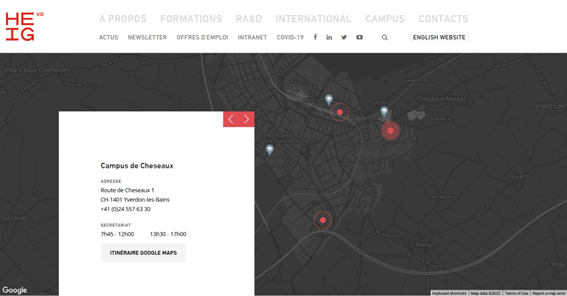
\includegraphics{actual_heig_plan.png}
    \caption{Plans actuels de la HEIG-VD}
    \label{fig:heigCurrentMap}
\end{figure}

La \gls{heig-vd} est une haute école dispensant des formations dans différents domaines de l'ingénierie, ainsi que de la gestion d'entreprise.
Elle se situe sur trois sites dispersés dans la ville d'Yverdon-Les-Bains, Vaud
: Cheseaux, en périphérie de la ville, St-Roch proche de la gare et le Y-Parc, dans la zone industrielle.

Cette école fournit sur son site web un plan \cite{plan-heig} (voir Figure \ref{fig:heigCurrentMap}) indiquant l'emplacement des trois bâtiments pricipaux.
On peut aussi y obtenir les informations sur les différents moyens d'accès à ces sites afin d'aider ses utilisateurs et  utilisatrices à s'orienter.
Cependant, elle ne fournit ni sur son site, ni dans le guide de l'étudiant, une interface permettant de s'orienter vers une salle ou une ressource précise.

\section{Description du problème}
M. Chevallier souhaite mettre à disposition des utilisateurs et utilisatrices une interface interactive pour permettre la visualisation des salles et des plans de la \gls{heig-vd} pour les trois bâtiments du campus.

\chapter{Analyse}
\section{Analyse fonctionnelle du système}
L'analyse fonctionnelle est un processus qui permet de déterminer les fonctionnalités d'un système à partir d'une analyse des besoins utilisateurs.

\subsection{Cas d'utilisation}
La première étape est de déterminer les cas d'utilisation du futur système.
Ceux-ci ont été établis lors de la conception du schéma des cas d'utilisation, Figure 2.1.
Celui-ci est en notation \gls{uml}, un des standards utilisés dans la modélisation d'application logiciel,
et a été réalisé à l'aide de l'application web \gls{diagrams} \cite{diagrams}.

\fig[width=7cm]{Schéma des cas d'utilisation}{useCaseDiagram.drawio.pdf}

Ce schéma présente les cas d'utilisation suivants :
\begin{itemize}
    \item Un utilisateur utilise le système pour s'orienter sur les différents sites de la HEIG-VD.
    \item Un utilisateur opère une recherche sur le système afin de localiser une ressource par des critères ou par son nom (une ressource est un terme générique pouvant symboliser une salle, l'emplacement d'un bureau d'un collaborateur, l'emplacement de matériel, etc.).
    \item Un utilisateur obtient des informations sur une ressource.
    \item Un utilisateur personnalise la carte et l'exporte pour d'autres usages.
\end{itemize}

\subsection{Analyse des besoins}
La deuxième étape de l'analyse fonctionnelle est de déterminer les besoins des utilisateurs à partir des cas d'utilisation du système.
Pour ce système, les besoins ont été déterminés dans la Table \ref{besoins}. Ils ont été numérotés de N1 à N8 pour pouvoir s'y référer plus facilement par la suite.
\begin{table}[h]
    \begin{center}
        \begin{tabular}{l|l}
               & Besoin                                                                                 \\ \hline
            N1 & S'orienter facilement à travers les sites de la HEIG-VD                                \\
            N2 & Localiser une ressource à l'aide de son nom                                            \\
            N3 & Localiser une ressource à l'aide de critères                                           \\
            N4 & S'informer efficacement sur une ressource                                              \\
            N5 & Être capable de personnaliser une carte                                                \\
            N6 & Être capable de partager sa carte personnalisée                                        \\
            N7 & S'informer efficacement des noms des noms des locaux, de leur surface, et de leur type \\
            N8 & Localiser facilement un collaborateur sur un plan des sites
        \end{tabular}
        \caption{Liste des Besoins \label{besoins}}
    \end{center}
\end{table}

\subsection{Fonctionnalités du système}
La troisième étape est de déterminer les fonctionnalités du système à partir des besoins des utilisateurs.
Ils ont été listés dans la Table \ref{fonctions}.
De plus, les besoins auxquels les fonctionnalités répondent dans la Table \ref{besoins} ont été précisés dans la colonne Besoins.
\begin{table}[h]
    \begin{center}
        \begin{tabular}{l|l|l}
                & Fonctionnalités                                                       & Besoins    \\ \hline
            F1  & Afficher un plan afin d'aider à l'orientation                         & N1, N7     \\
            F2  & Utilisable facilement et de façon ergonomique                         & N1         \\
            F3  & Fournir une orientation rapidement                                    & N1         \\
            F4  & Facilement accessible                                                 & N1         \\
            F5  & Afficher les ressources désirées                                      & N1, N3, N5 \\
            F6  & Fournir un outil de tracé du plus court itinéraire pour l'orientation & N1         \\
            F7  & Offrir un outil de localisation de ressource par nom                  & N2, N8     \\
            F8  & Fournir un outil de localisation de ressource par critère             & N3         \\
            F9  & Fournir des informations sur les ressources                           & N4, N7     \\
            F10 & Fournir un outil de dessin sur carte                                  & N5         \\
            F11 & Fournir un outil d'exportation                                        & N5         \\
            F12 & Fournir un outil d'impression de carte                                & N6         \\
            F13 & Fournir un outil de partage de carte                                  & N6         \\
            F14 & Fournir un outil de sauvegarde de carte                               & N6
        \end{tabular}
        \caption{Liste des Fonctionnalités \label{fonctions}}
    \end{center}
\end{table}

\section{Etat de l'art \Gls{websig}}
Dans cette section, différents systèmes d'interface web de visualisation de données géographiques (\gls{websig}) vont être analysés, ainsi que les technologies
associées à ce type d'application.

\subsection{\Gls{websig} existants}

\subsubsection{Plan EPFL}
\begin{figure}[h]
    \centering
    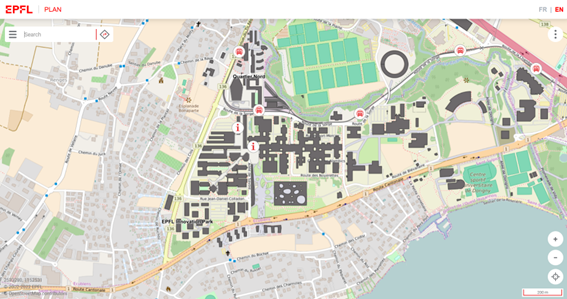
\includegraphics[scale=0.7]{planEPFL.png}
    \caption{Plans interactifs de l'EPFL}
\end{figure}

Les plans interactifs du campus de l'\gls{epfl} \cite{plan-epfl} affichent les bâtiments du campus en s'adaptant selon le zoom et l'étage sélectionné.
Suivant le zoom, on peut visualiser le contour du site, puis le contour des bâtiments et enfin les salles des bâtiments (voir \ref{fig:EPFLZoom}).

\begin{figure}[h]
    \centering
    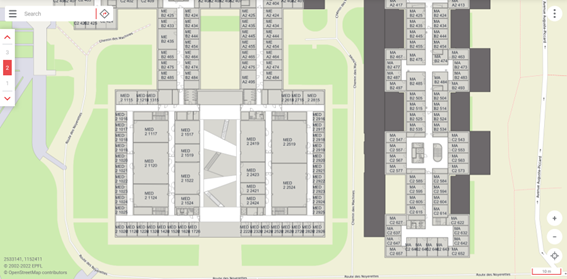
\includegraphics[scale=0.7]{planEPFLGrosPlan.png}
    \caption{Zoom sur les plans de l'EPFL }
    \label{fig:EPFLZoom}
\end{figure}

L'utilisateur a la possibilité de filtrer les points d'intérêts à afficher sur la carte à l'aide d'un menu sur la gauche du site.
Il y a aussi la possibilité de rechercher différentes ressources en fonction de leur nom, comme les bâtiments, les salles, les personnes, les restaurants, les magasins, ou encore les espaces culturels.
D'autres outils sont fournis, comme la recherche du plus court itinéraire entre deux ressources, un outil pour l'impression, ou un outil pour changer l'affichage pour une vue aérienne.
Finalement, un lien permet d'accéder au Géoportail de l'EPFL.

La principale technologie utilisée pour le frontend est Ngeo (combine Angular js et openlayers, plus de détails dans la section technologie).

\subsubsection{Géoportail EPFL}

\begin{figure}[h]
    \centering
    \includegraphics[scale=0.7]{géoportailEPFL.png}
    \caption{Géoportail de L'EPFL}
\end{figure}

Le Géoportail de l'EPFL \cite{geoportail-epfl} est très similaire au plan du campus, mais il offre la possibilité de dessiner des formes vectorielles sur la carte.
Il permet aussi d'afficher des ressources plus précises comme les réseaux wifi ou les prises électriques.

\subsubsection{MIT campus map}

\begin{figure}[h]
    \centering
    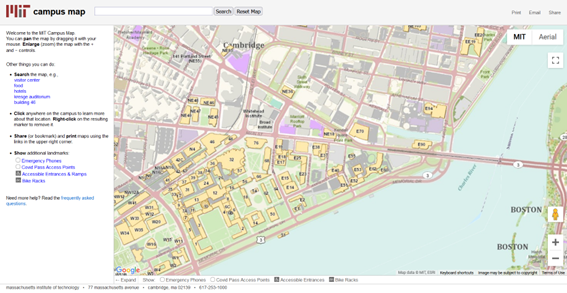
\includegraphics[scale=0.7]{MitCampusMap.png}
    \caption{Carte du campus du MIT}
\end{figure}

Les plans interactifs du MIT \cite{mit-map} affiche le tracé des bâtiments ainsi que le nom de ceux-ci. Seules les légendes s'adaptent en fonction du zoom.

Un utilisateur peut rechercher des bâtiments ou des points d'intérêts liés à l'université (ex : le world wide web consortium W3C).

Il peut aussi appliquer quelques filtres pour afficher des repères comme les restaurants. Cliquer sur un bâtiment permet d'obtenir des informations sur celui-ci. D'autres outils sont fournis comme un outil de partage ou d'impression.

L'affichage de la carte s'effectue à l'aide de l'API Google Maps, permettant un accès à Google Street View.

\subsubsection{SITN - Géoportail du système d'informations du territoire neuchâtelois}

\begin{figure}[h]
    \centering
    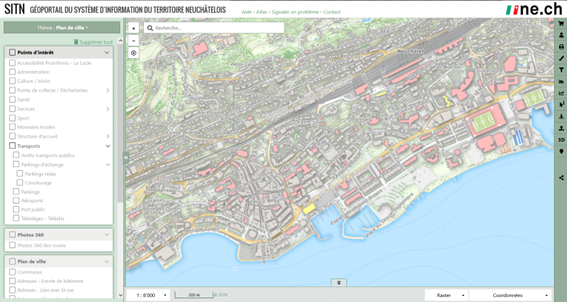
\includegraphics[scale=0.7]{planSITN.png}
    \caption{Plans du SITN}
\end{figure}

Les plans du SITN \cite{sitn} affichent les différentes informations géographiques du canton de Neuchâtel.
Le niveau de détail de la carte s'adapte en fonction du zoom.
Par exemple les numéros des maisons selon le cadastre de chaque commune s'affichent lors d'un zoom à une échelle 1 :1000.

Il y a la possibilité d'appliquer plusieurs filtres afin d'obtenir les informations recherchées comme le tracé des communes ou les points d'intérêts.

L'outil offre aussi des outils de dessin vectoriel, d'impression, la possibilité de changer le fond du plan, un accès à Google Street View, et un accès au géoportail LIDAR

Le site utilise GeoMapFish pour l'affichage des cartes ainsi que l'API Google Maps pour Google Street View.

\subsubsection{Stanford Campus Map}

\begin{figure}[h]
    \centering
    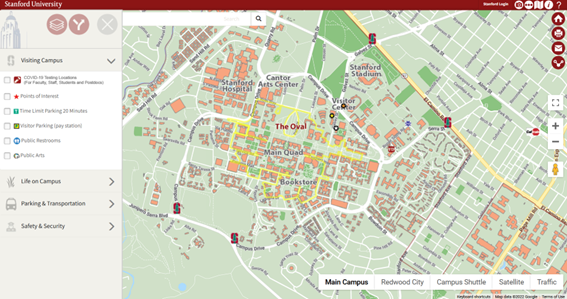
\includegraphics[scale=0.7]{standfordCampusMap.png}
    \caption{Plans du campus de Stanford}
\end{figure}

Le carte du campus de Stanford \cite{standford-map} affiche le tracé des bâtiments ainsi qu'une légende précisant le nom de ceux-ci.
Seul l'affichage de la légende varie selon lors d'un zoom rapproché.

Le site offre un outil de recherche de ressources aux utilisateurs, un accès à Google Street View, un outil d'impression et un outil de partage.

A noter que le menu en bas à droite est un mélange de plusieurs fonctionnalités, ce qui peut rendre l'utilisation confuse.

L'application web utilise l'API Google Maps pour l'affichage de la carte.

\subsubsection{Aéroport de Zurich}

\begin{figure}[h]
    \centering
    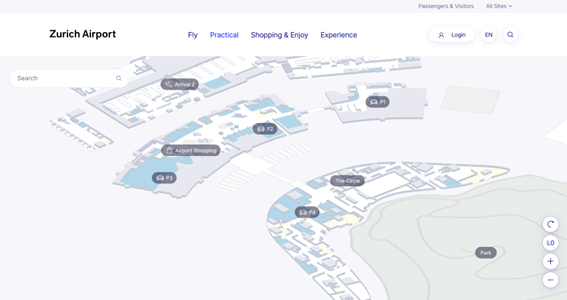
\includegraphics[scale=0.7]{planZurichAirport.png}
    \caption{Plans de l'aéroport de Zurich}
\end{figure}

L'aéroport de Zurich \cite{zurich-aeroport} offre un plan non géoréférencé en 3D isométrique.
Les différents points d'intérêts affichés varient en fonction du zoom.
L'application offre un outil de recherche avec des suggestions par thème.
On peut aussi changer le fond du plan en fonction de l'étage.

Les plans ne servent qu'à l'orientation des voyageurs et sont donc pauvre en fonctionnalités annexes.

Le site utilise le framework réactif React js, ainsi que le module bundler webpack. Les plans sont des images bitmap (pixellisées).

\subsection{Conclusions de l'analyse des systèmes existants}
On peut distinguer deux types d'applications :
des plans interactifs aidant les utilisateurs à s'orienter, ainsi que les Géoportails qui fournissent des informations géographiques
et permettent de construire de nouvelles données à l'aide d'outils de dessin vectoriel.

Cette distinction a été faite par l'EPFL qui distingue les deux types d'application dans deux sous-domaines.

Les technologies utilisées sont aussi différentes : les sites les plus complets utilisent souvent GeoMapFish alors que les sites les plus simples utilisent plutôt l'API Google Maps.


\subsection{Technologies pour les \gls{websig}}
Un \gls{websig} est une application web qui présente des données géographiques sur des plans.
Cette section présente plusieurs technologies qui facilitent la mise en place de tels systèmes.

\subsubsection{Openlayers}
Openlayers \cite{openlayers} est une librairie JavaScript open source qui aide à la construction d'applications \gls{websig}.
Elle permet de rajouter des calques contenant des données géographiques au-dessus d'un fond de carte.

\subsubsection{Leaflet}

Leaflet \cite{leaflet} est une librairie open source concurrente à Openlayers.
Elle est simple d'utilisation et légère.
On peut étendre la librairie à l'aide de plugins.

\subsection{Comparaison entre Leaflet et Openlayers}

\begin{table}[h]
    \begin{center}
        \begin{tabular}{l|c|c}
            Point de comparaison        & Leaflet        & Openlayers                      \\ \hline
            Simplicité d'utilisation    & simple         & moyen                           \\
            Poids                       & léger          & lourd                           \\
            Flexibilité                 & peu flexible   & très flexible                   \\
            Nombre de formats supportés & un seul format & plusieurs formats et protocoles \\
        \end{tabular}
        \caption{Tableau de comparaison entre Leaflet et Openlayers \label{compare}}
    \end{center}
\end{table}

On peut déduire que Leaflet est plus adapté à de petites applications ou applications mobiles \gls{websig} alors que openlayers est plus adapté à des applications plus complexes.

\subsubsection{Google Maps API}
L'API de Google Maps \cite{google-maps} n'est pas open source et peut être payante.
Elle n'offre pas la possibilité de rajouter des calques au fond de carte, mais uniquement des points d'intérêts.
Elle n'est donc pas adaptée à la construction d'applications \gls{websig}.

\subsubsection{GeoMapFish}
GeoMapFish est une technologie open source développée par l'entreprise camptocamp facilitant la construction de \gls{websig}.
Elle est composée de Ngeo pour le frontend \cite{ngeo} et de c2cgeoportal \cite{c2cgeoportal} pour le backend.

Ngeo est une librairie JavaScript basée sur le Framework réactif Angular Js et l'API Openlayers.

C2cgeoportal est la partie serveur construite à partir d'une image Docker. Il faut avoir des connaissances en Python pour l'utiliser.

Cette technologie est malheureusement obsolète car elle utilise une vieille version d'Angular qui est déconseillée pour le développement de nouveaux projets.

\subsubsection{PostGreSQL et PostGis}
PostGreSQL est une base de données relationnelle open source. Elle permet de stocker des données géographiques avec l'extension PostGis  \cite{postgis}.
Cette solution est utilisée par c2cgeoportal et dans de nombreuses autres applications \gls{websig}.

\section{Données existantes à disposition}
\subsection{Plans}
Des plans des étages des sites de Cheseaux et St-Roch non géoréférencés ont été fournis au format DGW, format propriétaire de AutoCAD, un logiciel de dessin technique.

\subsection{Serveur LDAP}
Un serveur LDAP est un service d'annuaire numérique.
La HEIG-VD possède un tel annuaire qui pourrait être utilisé pour acquérir des informations sur certaines ressources.

\chapter{Conception de la solution}

\section{Exigences de la solution}
Suite à l'analyse, nous pouvons établir qu'il faudra mettre en place une interface interactive de visualisation des plans comprenant uniquement le bâtiment de Cheseaux.
Celle-ci devra afficher toutes les salles du site avec leurs noms, un qualificatif (secrétariat, salle de cours, etc.) et leur surface en mètres carrés.
Un outil de changement d'étage permettra de parcourir les différents étages du site.
L'interface sera disponible tant sur de grand (télévision ) que sur de petit écran (téléphone mobile).

Cette application sera hébergée sur une machine virtuelle fournie par l'école.
Elle comportera une base de données qui s'occupera de stocker les données utilisées.
Un serveur API récupérera les informations et les enverra à l'utilisateur.

Elle positionnera aussi certaines ressources comme les collaborateurs sur le site de la HEIG-VD.

Si le temps le permet, un outil de filtrage des ressources à afficher et/ou un outil de recherche sera aussi développé.

La solution a pour but de démontrer les possibilités qu'elle offrirait à l'orientation des collaborateurs sur les différents sites de la \gls{heig-vd}.
Elle ne sera pas une solution utilisable par l'école.

\section{Solution envisagée}
Afin de répondre aux exigences, il a été défini que l'application sera un site web,
car c'est le moyen le plus accessible pour fournir cette interface, autant sur grand que petit écran,
et sans obliger l'utilisateur à télécharger un logiciel au préalable.

Elle sera contenue sur une seule page web (single-page application)
et offrira les différentes fonctionnalités à travers différents menus.
L'affichage se modifiera en fonction de son utilisation.

\section{Explications de certains principes}
Cette section explique les principes du web, d'un reverse-proxy, des containers et de la base de données.
Vous pouvez ignorer les sous-sections si vous avez des connaissances dans ces concepts.

\subsection{Web}
Il ne faut pas confondre internet, le standard qui régit la communication entre les ordinateurs
et le web qui se base sur internet et est utilisé par les navigateurs pour afficher des applications.
Le second utilise les protocoles de communications HTTP et HTTPS afin d'envoyer et récupérer des données.

Lorsqu'un utilisateur entre une URL, comme www.google.ch, dans un navigateur web, il va demander à un serveur de lui envoyer
plusieurs fichiers dans des formats différents afin de permettre l'affichage de l'application web.

Sont envoyés au navigateur des fichiers \gls{html} qui décrivent le contenu de l'application, des fichiers \gls{css} qui changent l'aspect de ce contenu,
des fichiers \gls{js}, un langage de programmation qui modifie le contenu selon les interactions de l'utilisateur avec l'application, et
les images à afficher.

En fonction de l'utilisation de l'application, celle-ci devra demander des données supplémentaires sur une ressource pour son fonctionnement.
Celles-ci sont envoyées dans des formats standardisés comme JSON ou XML.

\subsection{\Gls{rp}}
Un \gls{rp} est un serveur qui permet d'accéder à d'autres serveurs en utilisant la même url.
Cette machine va trier les requêtes des utilisateurs
et envoyer ces dernières sur le serveur correspondant le mieux.
Elle peut aussi refuser une requête si aucun serveur ne peut la traiter.
Utiliser un \gls{rp} amène aussi plus de sécurité car on n'expose pas les autres serveurs à l'extérieur.

\subsection{\Gls{container}}
Un container est une entité qui contient une application ainsi que les autres programmes nécéssaire à son fonctionnement.
Il est indépendant du système d'exploitation et permet d'installer les applications sur n'importe quelle machine en évitant les conflits provoqués par le système d'exploitation.
Pour exécuter un container, il faut au préalable installer un logiciel gérant ceux-ci sur le sytème d'exploitation.

On peut aussi créer des images de container. Celles-ci sont des fichiers regroupant les instructions qui permettent de construire les containers.
Elles peuvent être facilement dupliquées et partagées sur le web à travers des hébergeurs appelés container registry.

\subsection{Base de données}
Une base de données est un programme qui va organiser le stockage de données sur une machine.
Elle va simplifier l'obtention des données, l'ajout de nouvelles données, la modification et/ou la suppression de données existantes.

\section{Infrastructure}

\subsection{Architecture prévue}

L'infrastructure (voir Figure 3.1) tourne sur une machine virtuelle de la \gls{heig-vd} et est composée de quatre containers :

\fig[width=12cm]{Architecture de l'infrastructure}{infra.drawio.pdf}

\begin{itemize}
    \item Le reverse-proxy qui renvoie les requêtes vers le serveur ou le serveur-api.
    \item Le serveur qui envoie les fichiers \gls{html}, \gls{css}, et \gls{js} au client.
    \item Le serveur-api qui récolte les données depuis la base de données et les renvoie au client.
    \item La base de données qui stocke les informations.
\end{itemize}

Lorsqu'un utilisateur va demander l'accès à l'application en utilisant l'url "https://tb22-bourcoud.einet.ch/", il va accéder au reverse-proxy.
Celui-ci va renvoyer la requête vers le serveur.
Ce dernier sera chargé d'envoyer les fichier \gls{html}, \gls{css}, \gls{js} ainsi que les images au client en repassant par le reverse-proxy.

Par la suite, l'application a besoin d'obtenir les données des plans à afficher. Elle réaccède au reverse-proxy avec une adresse commençant par "https://tb22-bourcoud.einet.ch/api/",
et la requête est renvoyée au serveur-api. Ce dernier récolte les données demandées depuis la base de données et les renvoie au client en repassant par le reverse-proxy.

\subsection{Architecture idéale}
L'architecture mentionnée dans la sous-section précédente est valide pour ce travail de Bachelor.
Cependant, si l'école voulait mettre en place une solution plus aboutie,
il faudrait séparer chaque container dans des machines virtuelles différentes
et permettre aux serveur et serveur-api de se répliquer automatiquement
ou d'effacer des réplication en fonction du nombre d'accès à l'application (scalabilité horizontale élastique).
Cela permettrait aussi de faire face à la panne d'un des containers, car d'autres maintiendraient alors le service.

\section{Pipeline CI/CD}
Un pipeline CI/CD est une automatisation des opérations à exécuter sur les applications pour qu'elles soient mises à la disposition des utilisateurs.

\fig[width=12cm]{Pipeline CI/CD}{pipeline.drawio.pdf}

Le pipeline mis en place (voir Figure 3.2) va créer les images des containers du serveur et du serveur-api.
Les deux autres containers, vus à la section précédente, sont créés à partir d'images déjà disponibles.

Ce pipeline va d'abord tester les deux applications afin d'éviter que des problèmes surviennent.
Ensuite, il va construire les images et les publier sur un container registry.

\section{Technologies utilisées}

\subsection{\gls{node} et \gls{npm}}
\gls{node} est un programme qui permet d'utiliser le langage de programmation \gls{js} en dehors des navigateurs web.

Celui-ci est très utilisé chez les développeurs et possède de nombresuses librairies.

\gls{npm} est un programme qui gère les différentes librairies de \gls{node}.
Il permet d'ajouter, de mettre à jour, et de supprimer des librairies.

\subsection{\gls{ts}}
\gls{ts} est un langage de programmation reprenant comme base \gls{js} et lui ajoutant de nouvelles fonctionnalités utiles pour le développement.
Il se transforme (transpile) par la suite en \gls{js} lors de la construction de l'application web.

\subsection{\gls{vue3} composition}
\gls{vue3} est un framework \gls{js} permettant de simplifier l'écriture des interactions avec le contenu de l'application web.
Il est aussi chargé de créer du code \gls{html} et \gls{css} succeptible d'être facilement modifié.
Il offre deux styles d'écriture de code: composition ou option.
Ce projet a été écrit en utilisant le style "composition".

La librairie utilise une abstraction appelée "component" (mot anglais de composant) afin de créer les différents éléments de l'interface de l'application.

C'est un des frameworks les plus utilisés dans le développement d'applications web.
Il a l'avantage d'être plus complet et compréhensible que React, et nécessite aussi moins de code qu'Angular pour arriver à un résultat similaire.

\subsection{\gls{pinia}}
\gls{pinia} est une librairie associé à Vue 3 permettant de simplifier la communication de données entre les différents components.
Elle est conseillée par les développeurs de la librairie \gls{vue3} pour cette tâche.

\subsection{\gls{ol}}
\gls{ol} est une librairie JavaScript permettant d'implémenter des \gls{websig}.

\subsection{\gls{vite}}
\gls{vite} est un environnement de développement qui permet de simuler un serveur pour le développement en local,
et de construire (compiler) l'application tout en optimisant la place en mémoire qu'elle prendra.

Cet environnement est très vite installé et simplifie la compilation du programme.
Il permet aussi de créer un projet avec \gls{vue3} déjà intégré.

\subsection{\gls{vitest}}
\gls{vitest} est la librairie de test unitaire, conseillé par l'équipe de \gls{vue3} (permet de tester des parties du code indépendamment du reste).
Elle est optimisée pour fonctionner avec \gls{vite} mais peut être utilisée dans d'autres projets.

\subsection{\gls{vuetest}}
\gls{vuetest} est la librairie de test officielle de \gls{vue3} pour les components.

\subsection{\gls{nginx}}
\gls{nginx} est le serveur qui hébergera les fichiers HTML, CSS et JavaScript de l'application.

\subsection{\gls{express}}
\gls{express} est une librairie simplifiant la mise en place d'un serveur sur \gls{node}.
Il est utilisé pour créer le serveur-api.

\subsection{\gls{traefik}}
\gls{traefik} est le programme servant de \gls{rp} pour l'infrastructure du projet.
Il est plus simple à mettre en place par rapport à ses concurrents.

\subsection{\gls{postgres} et \gls{postgis}}
\gls{postgres} est la base de données utilisée pour le projet.
Elle est open source et peut être étendue par \gls{postgis}. Cette extension rajoute la possibilité de stocker des données géographiques.

\subsection{\gls{docker}}
\gls{docker} est le logiciel qui gérera les containers sur la machine virtuelle.


\subsection{\gls{git} et \gls{gitlab}}
\gls{git} est un programme permettant de facilement créer des versions du code source, revenir à une version précédente si besoin, et héberger son code sur des sites dédiés.

\gls{gitlab} est un hébergeur de code source utilisant l'utilitaire \gls{git}.
Il permet aussi la collaboration entre plusieurs développeurs sur une même application.

\subsection{\gls{cicd}}
\gls{cicd} est la fonctionnalité de l'hébergeur \gls{gitlab}
qui permet de lancer un pipeline CI/CD qui construira les deux images de container du projet.

\subsection{\gls{registry}}
\gls{registry} est l'hébergeur des deux images de container.


\section{Conception de la base de données}

\subsection{Base de données relationnelle}
Une base de données relationnelle est un type de base de données.
Au lieu de regrouper les données en une seule table,
elle permet d'en créer plusieurs et de former des liens entre elles.
Cela permet d'éviter la duplication de données.

A titre d'exemple, si on veut stocker tous les numéros de salle d'un bâtiment, tout en précisant à quel étage la salle appartient,
si on utilise une seule table la mention du nom de l'étage apparaitra sur plusieurs lignes.
Par contre, si on utilise une base de données relationnelle, on peut créer une table pour les salles,
une table pour les étages et former un lien entre les deux.

Cela permet aussi d'éviter les erreurs lors d'insertions de données.

\subsection{Schéma et choix}

\fig[width=12cm]{Schéma conceptuel de la base de données}{DB_model.drawio.pdf}

La conception de la base de données est représentée dans la Figure 3.3.
Ce schéma a été conçu en notation \gls{uml}. On y aperçoit les cinq tables qui seront décrites ci-après.
Si on étudie bien chaque table, on peut remarquer que certains champs auraient pu être séparés sur d'autres tables afin d'éviter des duplications.
Par exemple, le champ type dans room.

Il a été choisi de laisser ces duplications
car cela permet de simplifier le transfert de données géographiques sous format geoJson
(standard de fichier JSON pour le stockage de données géographiques).

\subsection{Tables et  relations}
\subsubsection{Building}
La table Building représente un bâtiment et est composée des champs suivants :

\begin{itemize}
    \item id : l'identifiant unique du bâtiment.
    \item name : le nom du bâtiment.
    \item x : la coordonnée x pour centrer le bâtiment sur une projection ESPG : 3857.
    \item y : la coordonnée y pour centrer le bâtiment sur une projection ESPG : 3857.
    \item ground\_floor : le nom de l'étage du rez-de-chaussée.
    \item rotation : la rotation par rapport au nord pour une meilleure visualisation du bâtiment.
    \item zoom : le zoom pour \gls{ol} pour une meilleure visualisation du bâtiment.
    \item min\_zoom : le zoom minimum pour \gls{ol} que pourra effectuer l'utilisateur.
    \item max\_zoom : le zoom maximum pour \gls{ol} que pourra effectuer l'utilisateur.
\end{itemize}

La table possède les relations suivantes :
\begin{itemize}
    \item Floor : le bâtiment possède plusieurs étage.
    \item Resource : le bâtiment peut posséder plusieurs ressources.
\end{itemize}

\subsubsection{Floor}
La table Floor représente un étage d'un bâtiment et est composée des champs suivants :

\begin{itemize}
    \item id : l'identifiant unique de l'étage.
    \item name : le nom de l'étage.
\end{itemize}

La table possède les relations suivantes :
\begin{itemize}
    \item Building : l'étage appartient à un bâtiment.
    \item Resource : l'étage peut posséder plusieurs ressources.
    \item Floor\_geometry : l'étage est composé de plusieurs données géométriques
\end{itemize}

\subsubsection{Floor\_geometry}
La table Floor\_geometry représente des données géométriques associées à un étage et est composée des champs suivants :

\begin{itemize}
    \item id : l'identifiant unique de la donnée géométrique.
    \item type : le type de géométrie.
    \item geometry : la donnée géométrique.
\end{itemize}

La table possède la relation suivante :
\begin{itemize}
    \item Floor : les données géométriques appartiennent à un étage.
\end{itemize}

\subsubsection{Room}
La table Room représente une salle d'un bâtiment et est composée des champs suivants :

\begin{itemize}
    \item id : l'identifiant unique de la salle.
    \item name : le nom de la salle (ex: E01).
    \item second\_name : le second nom de la salle s'il y en a un (ex: marketing). Il peut ne pas être renseigné.
    \item type : le type de salle (ex: salle de cours). Il peut ne pas être renseigné.
    \item area : la surface de la salle. Elle peut ne pas être renseignée.
    \item capacity : le nombre de places d'une salle. Il peut ne pas être renseigné.
    \item geometry : les données géométriques de la salle.
\end{itemize}

La table possède les relations suivantes :
\begin{itemize}
    \item Floor : la salle appartient à un étage.
    \item Resource : la salle peut posséder plusieurs ressources.
\end{itemize}

\subsubsection{Resource}
La table Resource représente tous types de ressources comme les extincteurs, les toilettes ou les ascenseurs
que l'on peut trouver dans un bâtiment, un étage, une salle. Elle est composée des champs suivants :

\begin{itemize}
    \item id : l'identifiant unique de la ressource.
    \item name : le nom de la ressource.
    \item type : le type de la ressource.
    \item image\_name : le nom de l'image associé à la ressource.
    \item description : la description de la ressource.
    \item localisation : la localisation de la ressource dans une projection ESPG : 3857.
\end{itemize}

La table possède les relations suivantes :
\begin{itemize}
    \item Building : la ressource est associée à un bâtiment.
    \item Floor : la ressource peut être associée à un étage.
    \item Room : la ressource peut être associée à une salle.
\end{itemize}

\section{Planification de la mise en place de la solution}
Ce chapitre présente la planification du projet et les principales étapes.

\subsection{Echéances et étapes}
Les principales échéances de ce travail sont le rendu d'un cahier des charges le jeudi 14 avril 2022,
le rendu d'un rapport intermédiaire le lundi 16 mai 2022,
le rendu final du projet initialement prévu le vendredi 29 juillet 2022 mais repoussé au vendredi 5 août 2022, et
finalement une défense qui aura lieu entre le 22 août et le 16 septembre 2022.

Il y a deux grandes étapes prévues :
une première version servant de proof of concept achevée le dimanche 29 mai 2022,
et la version finale du projet prévue pour le 29 juillet 2022.
Ces versions sont décrites dans les sous-sections suivantes.

D'autres versions pourront être mises en place par la suite afin de rajouter des fonctionnalités,
mais cela demanderait plus de temps que ce qui a été planifié pour le travail de Bachelor.

\subsection{Elaboration du projet}
La première étape consistait en l'analyse d'informations sur les projets \gls{websig}. Pour cela, 16 heures ont été planifées.
Ensuite, le travail consistait en la rédaction d'un cahier des charges et d'un planning. Pour ce faire, 25 heures ont été planifiées.

\subsection{Première version du projet}
La première étape était la prise en main des différentes technologies afin de vérifier la faisabilité du projet.
Le but était de mettre en place une application  \gls{websig} minimaliste n'affichant qu'un étage avec ses salles et n'offrant aucune fonctionnalité supplémentaire.

La réalisation de cette version nécessiterait de :

\begin{itemize}
    \item Traiter un des plans et créer les données géographiques (24 heures).
    \item Concevoir le design de l'application (8 heures).
    \item Mettre en place un pipeline CI/CD (4 heures).
    \item Création du serveur-api et de la base de données (16 heures).
    \item Création du frontend (24 heures).
\end{itemize}

\subsection{Deuxième version du projet}
La seconde étape mène à la mise en place de la solution finale.

La réalisation de cette version nécessiterait de :

\begin{itemize}
    \item Traiter les plans du site de Cheseaux et créer les données géographiques (54 heures).
    \item Mettre en place le serveur-api et de la base de données (30 heures).
    \item Mettre en place le frontend (70 heures).
    \item Déploiement de l'application sur la machine virtuelle (30 heures).
\end{itemize}

\subsection{Documentation du travail}
La documentation du travail étant importante, il a fallu planifier celle-ci:

\begin{itemize}
    \item Documentation du code (20 heures).
    \item Rapport intermédiaire (10 heures).
    \item Rapport final, (40 heures).
    \item Présentation (5 heures).
\end{itemize}

\section{Design de la solution}

Cette section décrit les designs imaginés pour la solution.
Ceux-ci ne sont pas précis et sont susceptibles de changer lors de l'implémentation.
De plus, des outils comme le menu de filtrage ou la recherche risquent de ne pas être implémentés.

\subsection{Design global}

\begin{figure}[h]
    \centering
    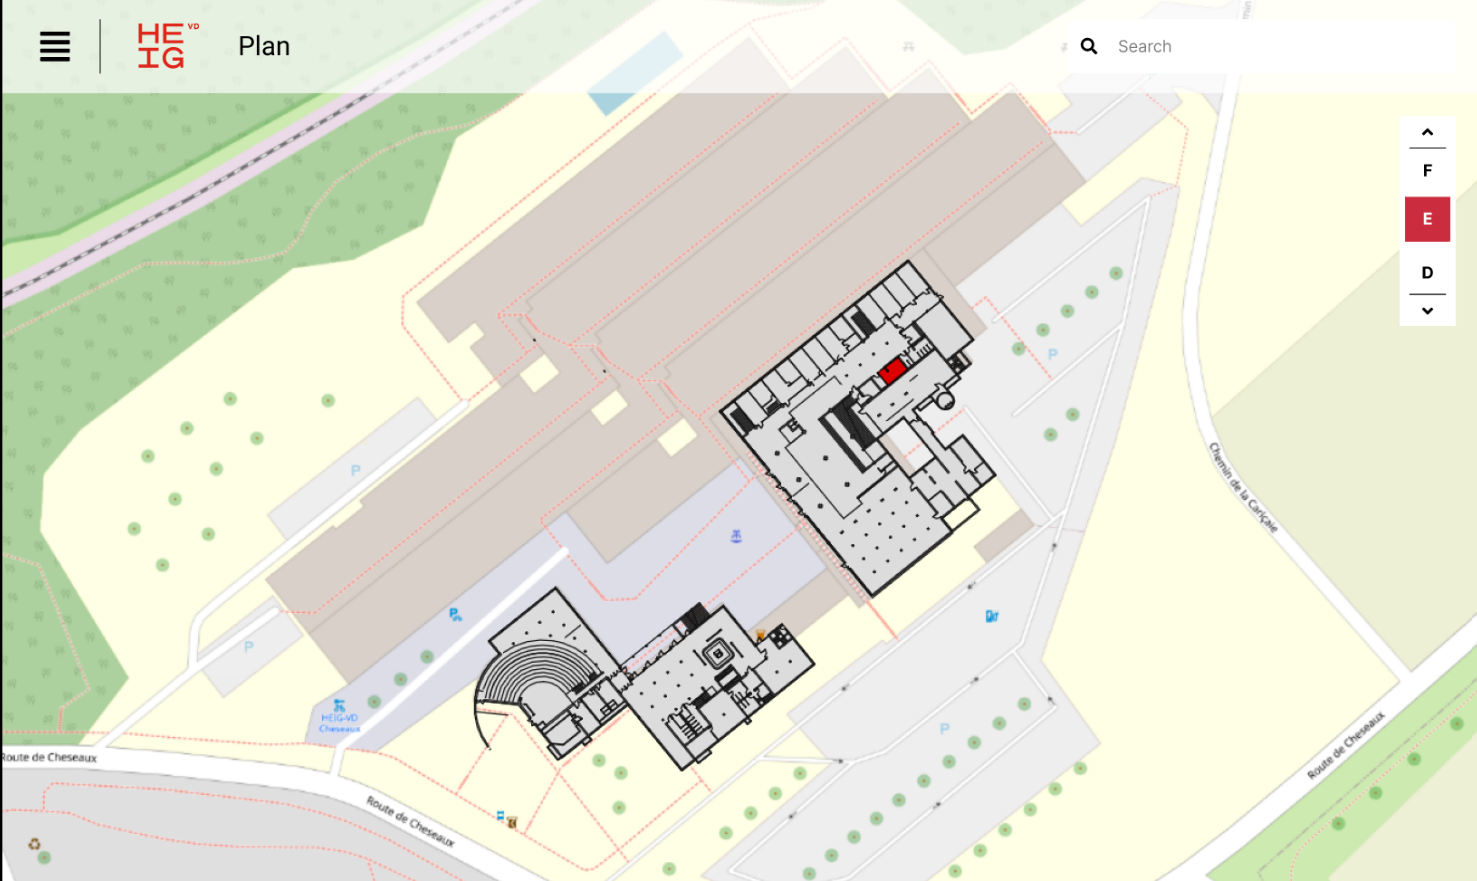
\includegraphics[scale=0.4]{designGlobal.png}
    \caption{Design global}
    \label{fig:globalDesign}
\end{figure}

Le design global (voir Figure \ref{fig:globalDesign}) tend à respecter la charte graphique du site heig-vd.ch/ en utilisant son logo, et son code couleur.
Le design a été conçu pour un écran au format 16/9, mais l'application sera aussi disponible pour d'autres types d'écrans.
L'application sera sur une seule page sans barre de défilement principal
(des barres de défilement secondaires seront possibles pour des fonctionnalités comme la fenêtre d'informations).

Cette page permet d'accéder à plusieurs outils :

\begin{itemize}
    \item Un menu pour filtrer les informations à afficher en cliquant sur le bouton en haut à gauche.
    \item Un outil de recherche à droite de l'en-tête.
    \item Un outil de changement d'étage à droite de la fenêtre.
    \item Une fenêtre d'informations en cliquant sur une salle ou en ayant effectué une recherche.
\end{itemize}

\subsection{Outil de changement d'étage}

\begin{figure}[h]
    \centering
    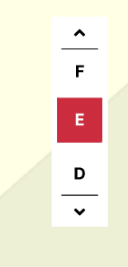
\includegraphics[scale=1]{designChangementEtage.png}
    \caption{Design de l'outil de changement d'étage}
    \label{fig:floorChange}
\end{figure}

L'outil de changement d'étage (voir Figure \ref{fig:floorChange}) permet de modifier l'étage affiché sur le plan.
Il indique, écrit en blanc sur fond rouge, l'étage actuel auquel se trouve l'utilisateur.
On pourra modifier celui-ci en cliquant sur les flèches.
L'outil indique également les étages adjacents
afin d'éviter une mauvaise utilisation de l'outil.

\subsection{Fenêtre d'informations}

\begin{figure}[h]
    \centering
    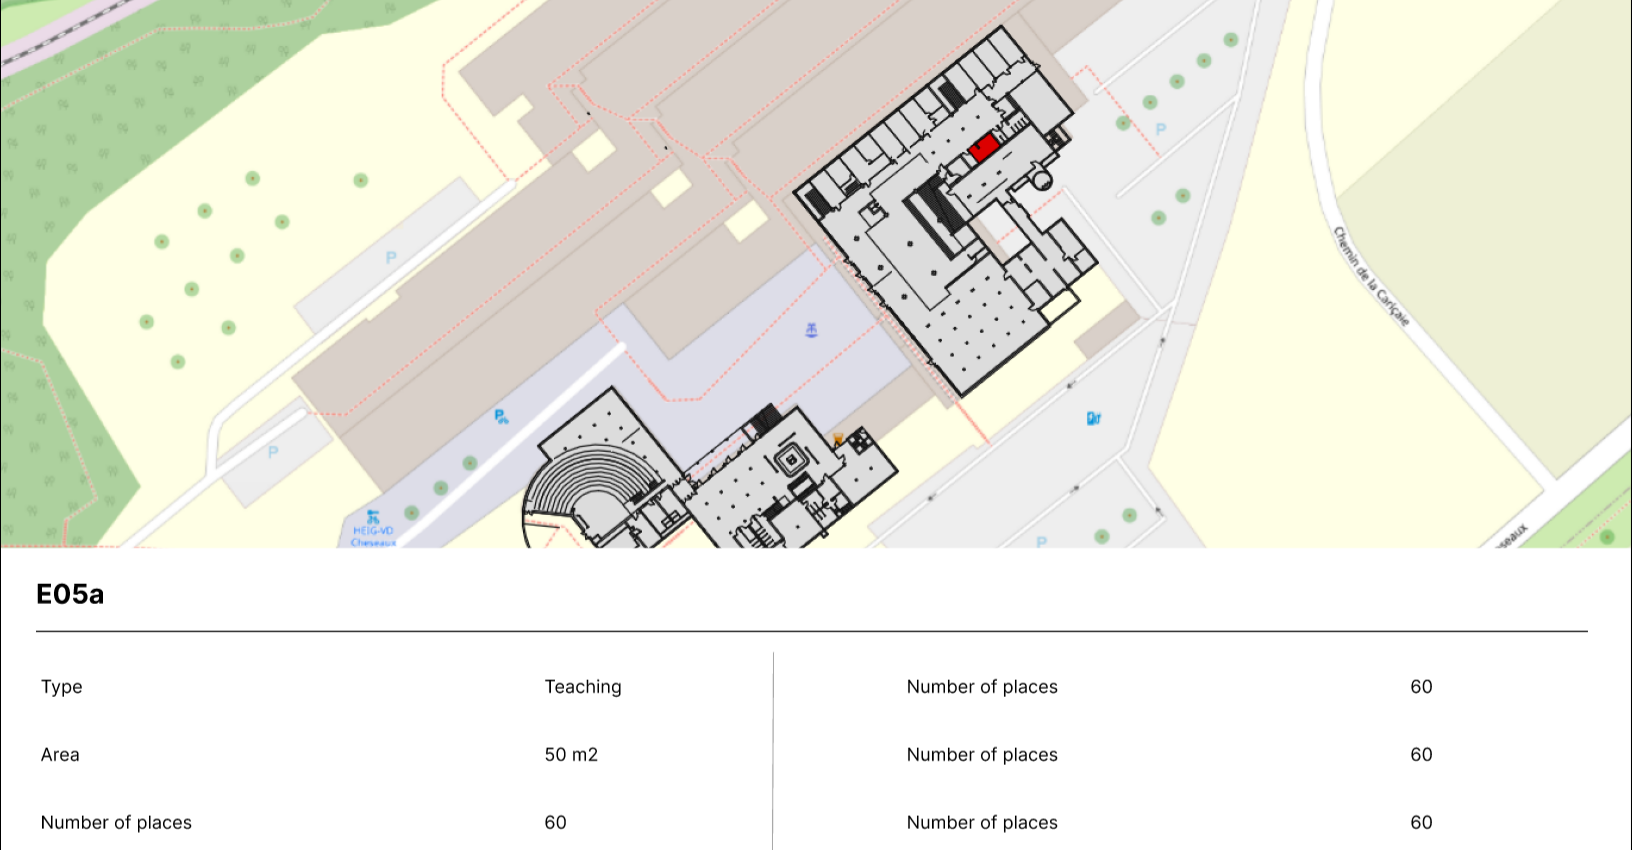
\includegraphics[scale=0.4]{designInfo.png}
    \caption{Design de la fenêtre d'informations}
    \label{fig:infoPanel}
\end{figure}

La fenêtre d'informations (voir Figure \ref{fig:infoPanel}) s'affichera sur le bas, lors d'un clic sur une salle ou après avoir exécuté une recherche.
Elle présentera les informations concernant la salle.
Pour la fermer, l'utilisateur pourra cliquer en dehors de la fenêtre.

\subsection{Menu de filtrage}

\begin{figure}[h]
    \centering
    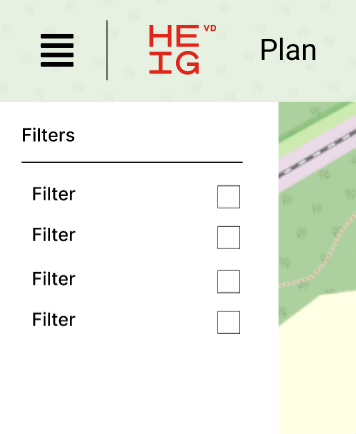
\includegraphics[scale=0.5]{designFilter.png}
    \caption{Design du menu de filtrage}
    \label{fig:filterPanel}
\end{figure}

Le menu de filtrage (voir Figure \ref{fig:filterPanel}) s'affichera sur la gauche de l'écran lorsque l'utilisateur cliquera sur le bouton en haut à gauche.
Il permettra d'ajouter ou de retirer des éléments à afficher sur la carte.
Pour sortir du menu, l'utilisateur pourra cliquer en dehors de celui-ci, ou à nouveau sur le bouton.

\subsection{Outil de recherche}

\begin{figure}[h]
    \centering
    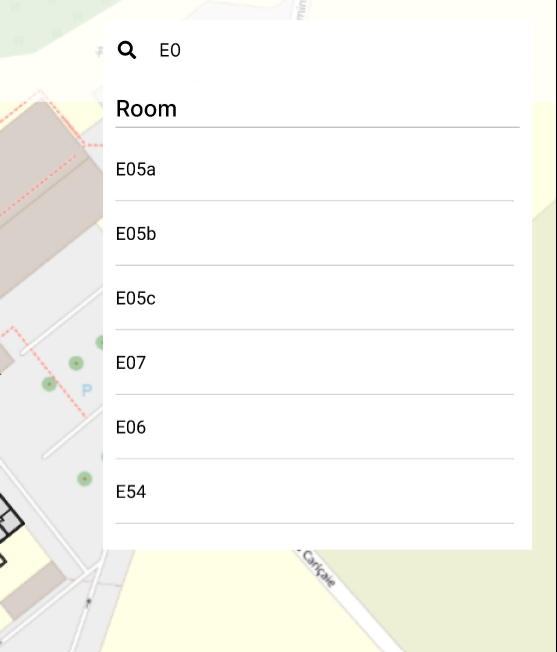
\includegraphics[scale=0.3]{designRecherche.png}
    \caption{Design de l'outil de recherche}
    \label{fig:searchBar}
\end{figure}

Lorsque l'utilisateur commencera à entrer des caractères dans le formulaire de recherche (voir Figure \ref{fig:searchBar}), celui-ci proposera un menu de suggestions.
Si l'utilisateur clique sur la touche entrée ou sur une des suggestions, l'affichage du plan se modifiera pour afficher la ressource demandée.


\chapter{Réalisation de la solution}

\section{Création des données géographiques}

Les données géographiques doivent être traitées, ou créées.
Cette section explique le processus de travail afin d'obtenir ces informations, ainsi que leur stockage dans la base de données.

La solution proposée dans cette section fera l'objet d'une critique dans le chapitre "Conclusion".

\subsection{\gls{qgis}}
\gls{qgis} est un logiciel de système d'informations géographiques qui permet de visualiser, traiter et diffuser ces informations.
Il a été utilisé dans ce projet afin de traiter les plans, et créer les autres données géographiques.

Une initiation à l'utilisation du logiciel a été nécéssaire afin de mettre en oeuvre une solution pour le projet.

\subsection{Les plans}
Les plans mis à disposition sont stockés dans des fichiers DWG, un format propriétaire du logiciel de dessin technique AutoCAD utilisé pour créer les plans d'architectes.
Ce format représente les informations géographiques en images vectorielles.
Les données sont séparées sur plusieurs calques.

Les plans ne sont pas encore géoréférencés, c'est-à-dire qu'ils se trouvent dans un système local de coordonnées
et qu'il faut les traiter afin de les placer dans un système de coordonnées exploitable par l'application.

\subsection{Géoréférencement des plans dans \gls{qgis}}
\begin{figure}[h]
    \centering
    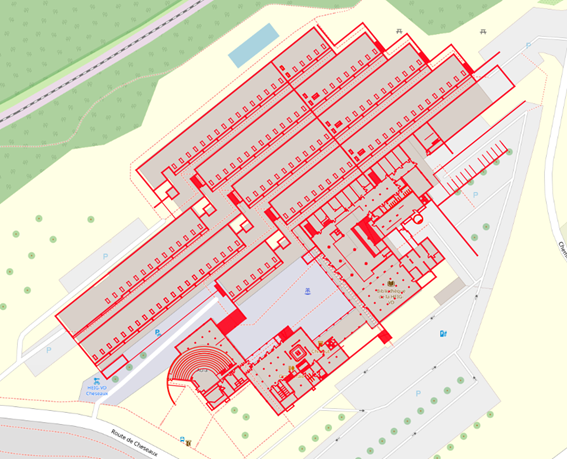
\includegraphics[scale=0.5]{Géoréférencement.png}
    \caption{Résultat final du géoréférencement d'un plan}
    \label{fig:georeferencement}
\end{figure}

Avant même d'ouvrir le logiciel \gls{qgis}, il faut choisir la projection (système de coordonnées) dans laquelle les plans seront géoréférencés.
Pour ce projet, la norme "ESPG : 3857 - WGS 84 / Pseudo-Mercator" a été choisie, car c'est celle utilisée par Open Street Map.

En premier lieu, il a fallu sélectionner les calques contenant les informations utiles au projet,
puis importer ceux-ci grâce à l'outil intégré dans \gls{qgis} "Import Layers from DWG/DXF".

En second lieu, il a fallu effectuer le géoréférencement.
Pour ce faire, le fond de carte Open Street Map a été intégré et servira de référence pour le placement des plans.
Le plugin "Vector Bender" a été utilisé pour effectuer une transformation affine sur les plans afin de les déplacer vers la bonne référence.
Finalement. les nouvelles données ont été enregistrées au format "ESRI shapefile", plus adapté au manipulations dans ce logiciel.

Le résultat final peut être observé à la Figure \ref{fig:georeferencement}.

\subsection{Création des informations géographiques}

\begin{figure}[h]
    \centering
    \includegraphics[scale=0.6]{créatioNgeodata.png}
    \caption{Résultat final de la création d'informations de l'étage E}
    \label{fig:polygones}
\end{figure}

Une fois le géoréférencement fini, seul le tracé de chaque étage était visible.
Il a fallu ensuite créer les données suivantes :

\begin{itemize}
    \item Le contour des étages sous forme de polygones au lieu de lignes.
    \item Le contour des salles sous forme de polygones.
    \item La localisation des ressources sous forme de points.
\end{itemize}

La Figure \ref{fig:polygones} illustre la création du contour de l'étage E et de ses salles.
La Figure \ref{fig:ressources} illustre la création de localisations des ressources.

Le travail de création des données géographiques pour le site de Cheseaux a été chronophage.

Lors de la création de ces données, il y a la possibilité de rajouter des métadonnées à chaque information géographique
(données supplémentaires). Cependant, ce travail a été principalement effectué sans avoir dans son optique cette possibilité.
Une rectification nécessiterait un temps considérable.


\begin{figure}[h]
    \centering
    \includegraphics[scale=0.6]{data-créationRessources.png}
    \caption{Résultat final de la création d'informations des ressources}
    \label{fig:ressources}
\end{figure}

\subsection{Problèmes rencontrés avec \gls{qgis}}
Le premier problème rencontré lors de l'utilisation du logiciel concernait les recherches de solutions pour le géoréférencement,
certains outils ne faisant pas de transformation affine correcte ou émettant des erreurs.

Le second concernait le plugin "Vector Bender", nécessitant alors que tous les calques utilisés pour la transformation affine utilisent la même projection.

\subsection{Exportation et arborescence de fichiers}
Afin de pouvoir traiter les données et les placer dans la base de données,
il fallait exporter celles-ci depuis le logiciel dans un format facilement lisible par un programme informatique.
Le choix s'est porté sur le format \gls{geojson}.

Celles-ci ont été exportées dans l'arborescence de fichiers suivante.

Le dossier racine contient des dossiers portant le nom des différents bâtiments.
Ces derniers contiennent des dossiers portant le nom de chaque étage ainsi qu'un dossier contenant les fichiers \gls{geojson} des ressources liées au bâtiment.
Les dossiers des étages contiennent les fichiers \gls{geojson} des informations géographiques relatifs à l'étage, ainsi qu'un dossier portant le nom rooms.
Ce dernier contient les fichiers \gls{geojson} relatifs à chaque salle.

Cette arborescence sera utile pour la création des scripts SQL.

\subsection{Création des scripts SQL}
SQL est un langage permettant la gestion de bases de données relationnelles comme \gls{postgres}.
Celui-ci permet de créer la base de données ainsi que les tables, de récupérer les données, d'en insérer de nouvelles, d'en modifier ou d'en supprimer.

Pour ce projet, un programme  a été créé afin de lire les fichiers dans l'arborescence décrite dans la sous-section précédente
et créer trois fichiers SQL : un pour la création de la base de données ; un pour la création des tables ; un pour l'insertion des données géographiques.

Ils seront utilisés afin de mettre en place la base de données lors du déploiement de l'application.

\section{Backend | Serveur-api}
Le serveur-api s'occupe de récupérer les données depuis la base de données, et de les envoyer à l'application web.

\subsection{Organisation du code source}

\begin{figure}[h]
    \centering
    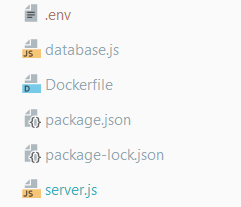
\includegraphics[scale=0.9]{backend_source_code.png}
    \caption{Arborescence de fichiers du serveur-api}
    \label{fig:backend_source_files}
\end{figure}

La Figure \ref{fig:backend_source_files} contient deux fichiers importants: server.js qui implémente le serveur \gls{express} et les différentes routes,
et database.js qui contient le code de connection à la base de données et les requêtes SQL pour les acheminer.

\subsection{Communications}

\fig[width=12cm]{Diagramme de séquence représentant les communications pour le serveur-api}{serverApi_sequenceDiagram.drawio.pdf}

Le diagramme de la Figure 4.5 présente les communications entre le client web,
le serveur-api, et la base de données. Le client web va d'abord faire une requête HTTP au serveur-api.
Ce dernier va envoyer une requête SQL à la base de données afin de récupérer les informations utiles.

Lorsque qu'il reçoit les informations, il va vérifier si celles-ci sont existantes.
Le cas échéant, il va les traiter puis les envoyer en format JSON au client web, avec le code de statut "200 OK", propre au protocole HTTP.
Dans le cas contraire, il va retourner un message d'erreur avec le code de statut "400 Bad request".

\subsection{Routing}

L'application web a besoin d'acheminer différentes ressources. Pour ce faire, elle accède au serveur-api en utilisant différentes URLs liées aux données désirées.
Ces URLs sont appelées routes.

Les routes seront présentées avec la deuxième partie de l'URL.
Par exemple, le site factice www.site.web/element1/:element2 sera présenté seulement avec /element1/:element2.

De plus, si un des éléments est précédé par deux points, cela veut dire qu'il peut prendre n'importe quelle valeur.
Par exemple, /element1/:element2 peut être écrit /element1/356 ou /element1/bonjour.
Cette valeur sera utilisée lors de la requête SQL et récupérera les informations correspondant aux entrées de la base de données.

Ci-dessous la liste de chaque route et des données récupérées :

\begin{itemize}
    \item '/api/buildings' récupère les informations sur tous les bâtiments.
    \item '/api/buildings/:buildingId/floors' récupère les informations sur les étages d'un bâtiment.
    \item '/api/buildings/:buildingId/resources' récupère les informations sur les ressources liés à un bâtiment mais pas à un étage.
    \item '/api/floors/:floorId/features' récupère les informations liées à un étage.
    \item '/api/rooms/:roomId/resources' récupère les ressources liées à une salle.
    \item '/api/rooms/search/:search' récupère les noms des salles selon une recherche.
    \item '/api/rooms/:name' récupère les informations d'une salle selon leur nom.
\end{itemize}

\subsection{ORM}
Ce projet n'utilise pas d'ORM,
une technique de programmation qui facilite la récupération de données prêtes à l'emploi, pour les raisons suivantes :
\begin{itemize}
    \item Les données sont récupérées au format JSON, utilisable par le langage de programmation \gls{js} sans trop de transformation.
    \item Certaines requêtes sont spécifiques à l'extension \gls{postgis} et auraient demandé d'étendre les fonctionnalités de l'ORM.
    \item Le serveur-api ne fait que peu de traitement de données avant de les renvoyer au client web.
\end{itemize}



\section{Frontend}

Le frontend est un projet qui sera transformé en fichier \gls{html}, \gls{css} et \gls{js}, avant d'être délivré par le serveur.

\begin{figure}[h]
    \centering
    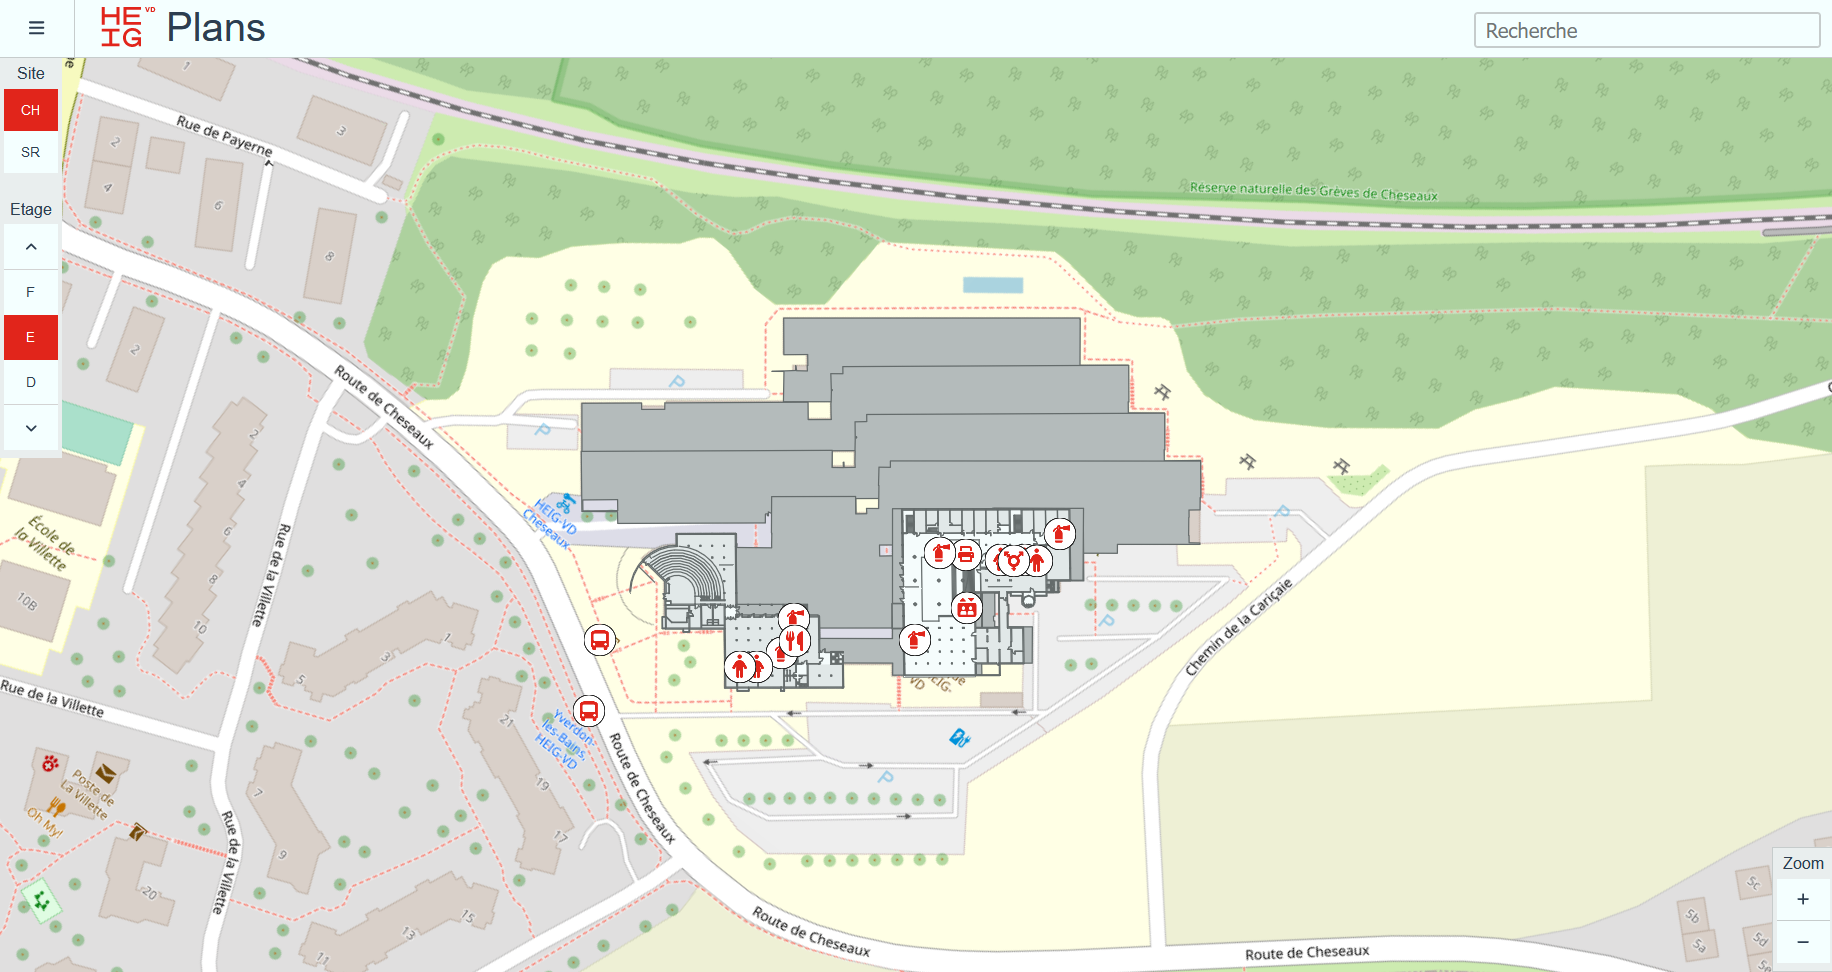
\includegraphics[scale=0.3]{frontend-global.png}
    \caption{Affichage global de l'application}
\end{figure}

\subsection{Organisation du code source}

\begin{figure}[h]
    \centering
    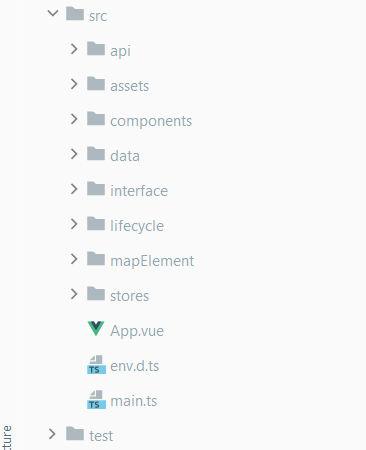
\includegraphics[scale=0.7]{frontend-source-organisation.png}
    \caption{Organisation du code source}
    \label{fig:fichier-source}
\end{figure}

Le code de l'application (voir Figure \ref{fig:fichier-source}) se trouve dans le dossier nommé "src" (abréviation de source), et les tests dans le dossier test.
A la racine du dossier "src" se trouve le fichier "main.ts", porte d'entrée de l'application,
ainsi que le fichier "app.vue", component Vue principal qui englobe tous les autres components.

Le reste du dossier est composé des dossiers suivants :
\begin{itemize}
    \item api : contient le code permettant de communiquer avec le serveur-api.
    \item assets : contient les images de l'application.
    \item component : contient les components Vue, organisés dans des sous-dossiers par type de component.
    \item interface : contient les interfaces \gls{ts} qui définissent des types d'objet.
    \item lifecycle : contient le code gérant la stratégie de récolte des données.
    \item mapElement : contient les élements concernant la librairie \gls{ol}.
    \item stores : contient les fichiers permettant de communiquer des informations entre plusieurs component Vue.
\end{itemize}

\subsection{Stratégie de récupération des données}

\fig[width=12cm]{Schéma de la stratégie de récupération des données}{frontend_flowChart.drawio.pdf}

La récolte des données nécéssaires au bon fonctionnement de l'application se fait en deux temps(voir Figure 4.8).
Ceci permet à l'utilisateur d'accéder plus rapidement à l'application sans devoir attendre que celle-ci soit complétement prête.
Dans un premier temps, l'application va récupérer les données nécéssaires via le serveur-api
afin d'afficher le fond de carte, l'étage E de Cheseaux et les ressources associées à cet étage.
L'utilisateur pourra alors accéder aux plans sans trop d'attente.

Dans un deuxième temps, le serveur-api va récupérer les informations géographiques de tous les bâtiments contenues dans la base de données,
ainsi que leur étage.

Toutes les données récupérées lors de ces deux étapes sont mises en cache (stockées temporairement sur la machine de l'utilisateur),
afin d'éviter de multiplier les requêtes, et permettre ainsi une navigation fluide sur la carte sans temps de latence.

Lors de l'utilisation de l'outil de recherche, des requêtes sont encore effectuées pour récupérer les données de salle.

\subsection{\gls{ol} calques}
\gls{ol} permet de séparer les données géographiques sur plusieurs calques (layers) superposés.
Afin d'afficher les plans, les données géographiques ont été séparées sur les calques suivants :

\begin{itemize}
    \item osmLayer : calque affichant le fond de carte fourni par Open Street Map.
    \item backgroundLayer : calque affichant les contours du bâtiment.
    \item polygonLayer : calque affichant le fond de l'étage sélectionné.
    \item lineLayer : calque affichant les lignes provenant du plan de l'étage selectionné.
    \item labelsLayer : calque affichant les noms des salles.
    \item resourceLayer : calque affichant les icones des ressources.
\end{itemize}

Quand un utilisateur veut changer d'étage ou de bâtiment, les sources de données des calques sont remplacées par d'autres sources.

\subsection{Fonctionnalités}

\subsubsection{Ecran de chargement}

\begin{figure}[h]
    \centering
    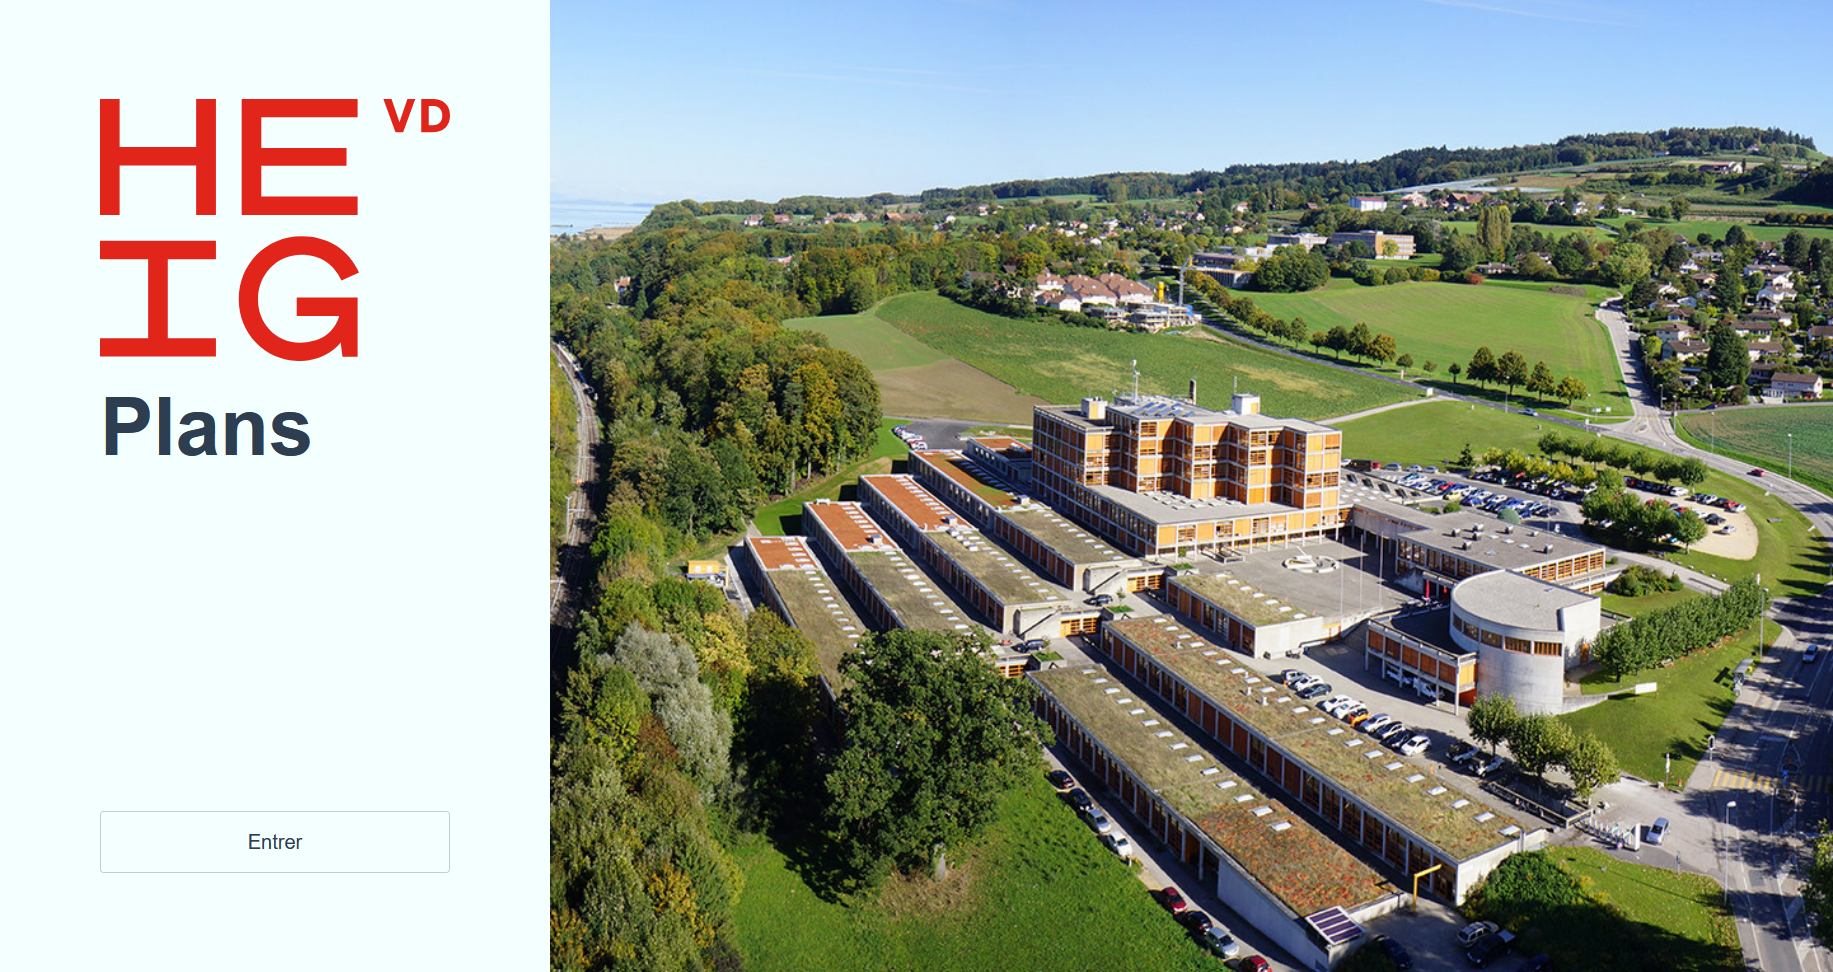
\includegraphics[scale=0.3]{frontend-loading-screen.png}
    \caption{Ecran de chargement}
    \label{fig:ecran-chargement}
\end{figure}

L'écran de chargement (voir Figure \ref{fig:ecran-chargement}) permet de faire patienter l'utilisateur jusqu'au chargement des informations essentielles à l'affichage des plans
(1ère étape de la récupération des données).
Il permet aussi de donner un aperçu du bâtiment de Cheseaux et ainsi offrir une meilleure compréhension des plans par la suite.

L'accès aux plans se fait au moyen d'un bouton.

\subsubsection{Outil de changement de bâtiment}

\begin{figure}[h]
    \centering
    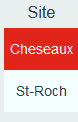
\includegraphics[scale=0.8]{frontend-buildingChange.png}
    \caption{Outil de changement de bâtiments}
    \label{fig:changement-batiment}
\end{figure}

L'outil de changement de bâtiment (voir Figure \ref{fig:changement-batiment}) permet de naviguer d'un bâtiment à l'autre.
Le bâtiment actuellement selectionné est écrit en blanc sur fond rouge. Les autres bâtiments sont des boutons.
Tous les textes  sont des abréviations des noms des bâtiments, et lorsque l'utilisateur passe le curseur au dessus de l'outil,
le nom entier s'affiche à la place des abréviations.

Lors d'un clic sur un des ces boutons, le plan change d'affichage et se centre sur le bâtiment nouvellement sélectionné.
Les sources des calques sont modifiées en conséquence.
L'étage qui est selectionné est le rez-de-chaussée du bâtiment, mentionné dans la base de données.
L'outil de changement d'étage adapte aussi la liste des étages.
Cependant, ceci ne se vérifie pas dans la version finale car les données des étages de St-Roch ne sont pas implémentées,
le comportement normal de l'application lors de données manquantes étant de ne pas modifier la liste.

Lors de la conception du design, cet outil n'avait pas été planifié.

\subsubsection{Outil de changement d'étages}

\begin{figure}[h]
    \centering
    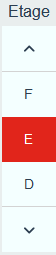
\includegraphics[scale=0.8]{frontend-floorChange.png}
    \caption{Outil de changement d'étages}
    \label{fig:changement-étage}
\end{figure}

L'outil de changement d'étages (voir Figure \ref{fig:changement-étage}) permet de naviguer à travers les étages d'un bâtiment.
Il présente l'étage selectionné, ainsi que les étages adjacents.

Le design de l'outil correspond à ce qui était prévu. Il a cependant été associé a l'outil de changement de bâtiment dans une barre d'outil,
et a été placé à gauche.

\subsubsection{Outil de filtrage des ressources}

\begin{figure}[h]
    \centering
    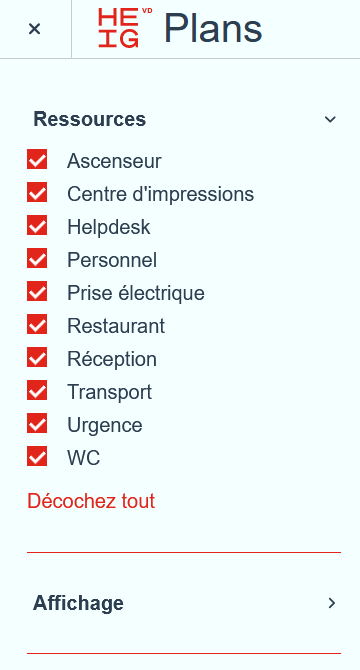
\includegraphics[scale=0.5]{frontend-filtresRessources.png}
    \caption{Outil de filtrage des ressources}
    \label{fig:ressources-filtre}
\end{figure}

L'outil de filtrage des ressources (voir Figure \ref{fig:ressources-filtre}) se trouve dans le menu accessible à partir du bouton à gauche du header.
Il permet de sélectionner les types de ressources à afficher.
Si ces dernières sont sélectionnées, les icones des ressources correspondantes s'affichent sur le plan.
Dans le cas contraire, les icones sont masquées.

Le design de l'outil est plus abouti que la conception initiale : les cases à cocher se trouvent à gauche, et
il se trouve dans un menu déroulant.

\subsubsection{Outil de changement d'affichage}

\begin{figure}[h]
    \centering
    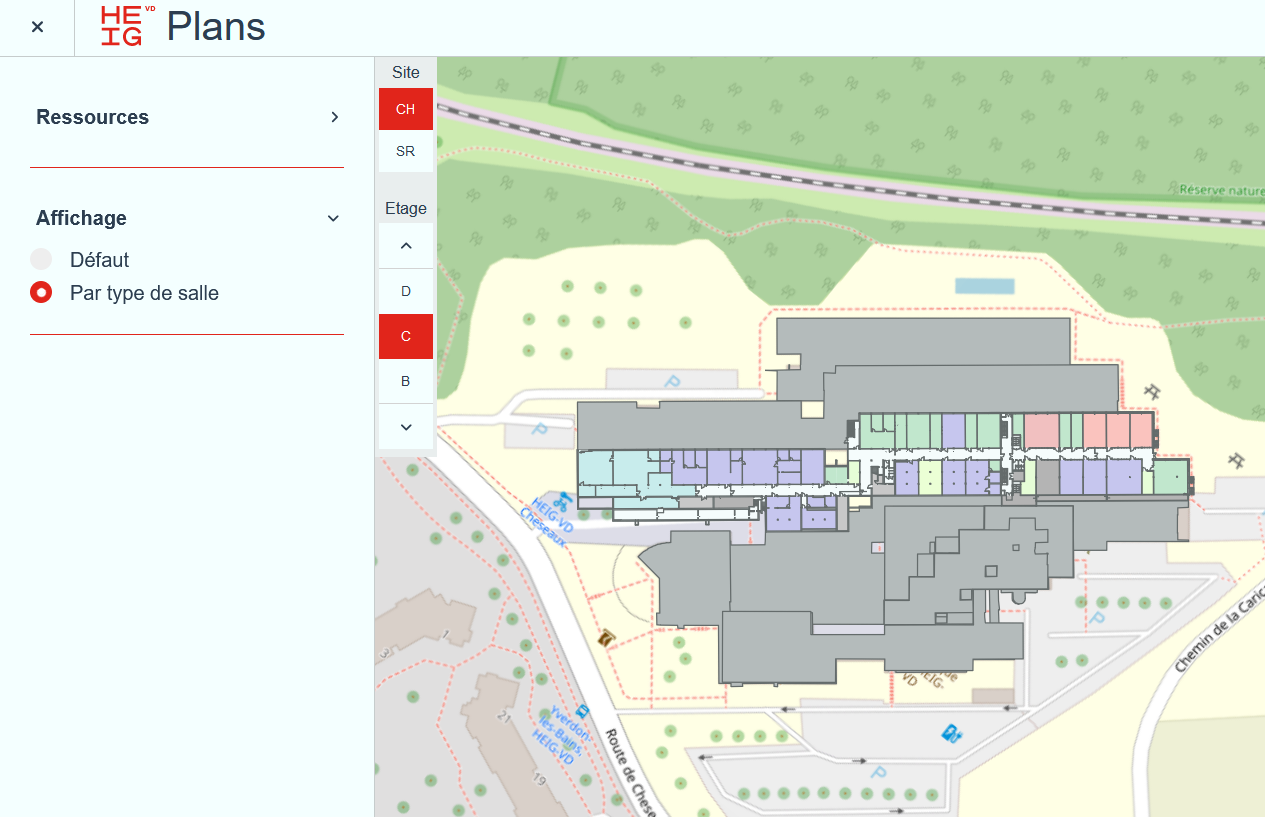
\includegraphics[scale=0.4]{frontend-affichageParType.png}
    \caption{Outil de changement d'affichage et effet sur les plans}
    \label{fig:affichage}
\end{figure}

L'outil de changement d'affichage (voir Figure \ref{fig:affichage}) permet de modifier la présentation des plans.
Actuellement, deux affichages différents sont disponibles :
celui par défaut, et un affichage qui colorise les salles en fonction de leur type.

Lors de la conception du design, cet outil n'avait pas été planifié.

\subsubsection{Interaction avec les plans}
L'utilisateur peut interagir avec les plans en cliquant sur des salles ou des icones de ressources.
Si c'est le cas, celles-ci se mettent en mode sélectionné et l'application affiche la fenêtre d'informations.

Cela est possible car \gls{ol} fournit des évènements lors de l'interaction avec les plans.

Grâce à \gls{ol}, il est possible de sélectionner plusieurs salles ou ressources en maintenant la touche shift.
Ceci est géré par la fenêtre d'informations en affichant les infos de chaque salle ou ressource.

\subsubsection{Outil de recherche}

\begin{figure}[h]
    \centering
    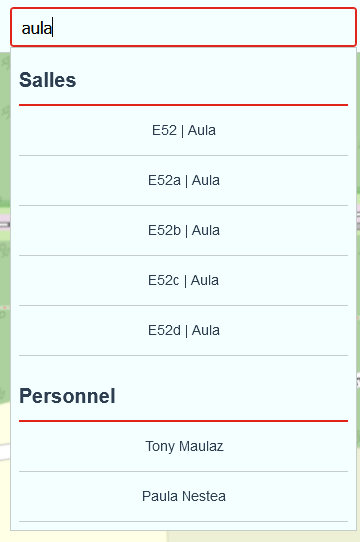
\includegraphics[scale=0.5]{frontend-recherche.png}
    \caption{Outil de recherche avec menu des suggestions}
    \label{fig:recherche}
\end{figure}


L'outil de recherche (voir Figure \ref{fig:recherche}) permet de rechercher une salle par son numéro ou par son nom.
Il permet aussi de trouver la salle où se trouve un collaborateur de l'école en écrivant son nom.

A partir de deux caractères écrits, l'outil propose des suggestions de salles et/ou de collaborateurs.
L'utilisateur peut cliquer sur une des suggestions.
S'il le fait, les plans change pour afficher la salle concernée en rouge et les informations de celle-ci dans la fenêtre d'informations.

Si l'outil n'a aucune suggestion à proposer, il affiche une erreur.
Si l'utilisateur clique sur un collaborateur lié à une salle non implémenté dans la base de données,
un message d'alerte le précise à l'utilisateur.

Lorsque l'utilisateur clique en dehors de la barre de recherche, le menu de suggestions disparait,
et reapparait lorsqu'il reclique à l'intérieur.

Afin de limiter les requêtes au serveur-api, les données des salles sont mises en cache à partir de deux caractères.
Ce cache est réinitialisé quand l'utilisateur clique sur une suggestion, ou qu'il efface sa saisie en dessous de deux caractères.

Le design de l'outil n'est pas très différent de la conception initiale : l'icone de loupe n'apparaît plus dans la barre de recherche.
Les suggestions de salle proposent en plus du numéro le nom de la salle.

\subsubsection{Fenêtre d'informations}

\begin{figure}[h]
    \centering
    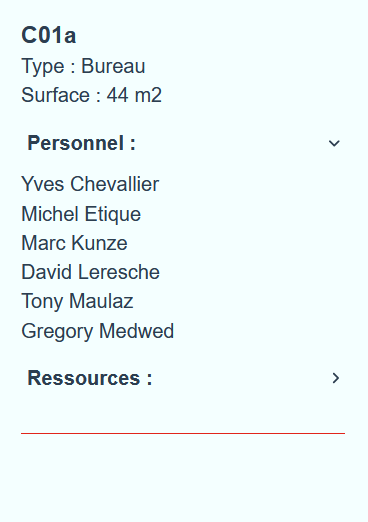
\includegraphics[scale=0.5]{frontend-info.png}
    \caption{Fenêtre d'informations}
    \label{fig:info}
\end{figure}

La fenêtre d'informations (voir Figure \ref{fig:info}) peut apparaître soit après une recherche, soit lors d'une interaction avec les plans.
Celle-ci fait apparaître toutes les informations disponibles au sujet de la salle ou de la ressource.
Dans le cas d'une salle, il peut afficher dans une liste déroulante le personnel
et/ou les ressources associées à celle-ci.

Pour quitter la fenêtre d'informations, il faut cliquer directement sur les plans.

\subsection{Responsivité}

\begin{figure}[h]
    \centering
    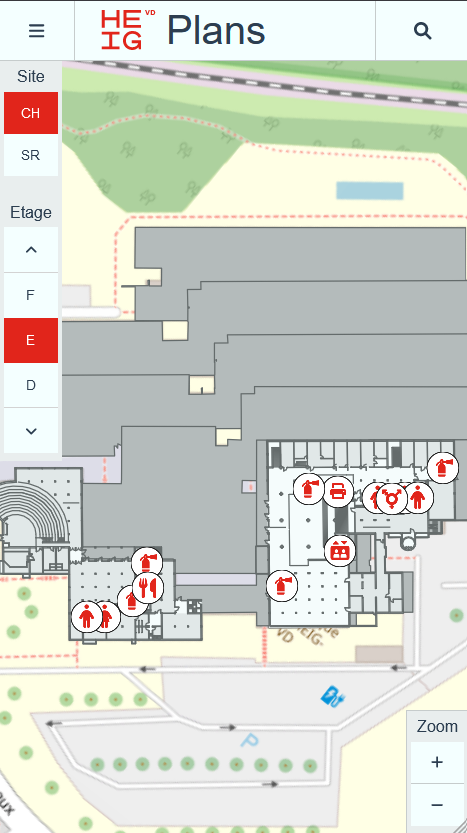
\includegraphics[scale=0.5]{frontend-responsive-portrait.png}
    \caption{Affichage sur smartphone en mode portrait}
\end{figure}

Afin de garantir l'accessibilité des fonctionnalités lors de l'utilisation de l'application,
l'affichage s'adapte en fonction de la taille de l'écran.

Si la largeur de l'écran est trop petite, la barre de recherche devient un bouton avec une icone de loupe.
Si l'utilisateur clique dessus, le barre de recherche s'affiche à la place du logo et du titre de l'application.
Celui-ci redevient normal lorsque l'utilisateur reclique sur le bouton ou finalise sa recherche.

La fenêtre d'informations s'adapte aussi si la largeur est trop petite.
Elle s'affiche au bas de l'écran au lieu de la droite.

Si la hauteur de l'écran est trop petite, le menu comportant les outils de changement de bâtiment et d'étages
se place sur deux colonnes.

\begin{figure}[h]
    \centering
    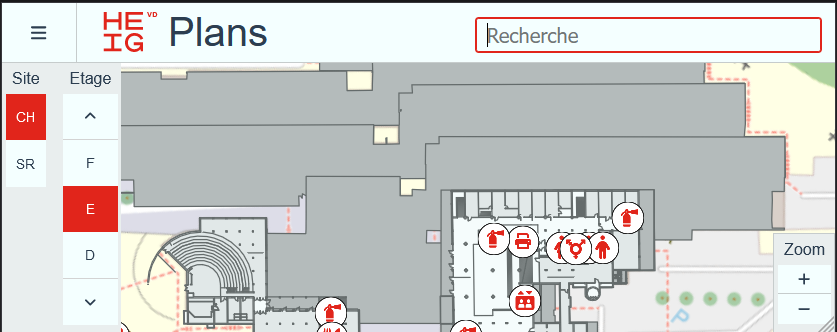
\includegraphics[scale=0.5]{frontend-responsive-paysage.png}
    \caption{Affichage sur smartphone en mode paysage}
\end{figure}

\section{Déploiement}

\subsection{Docker compose}
Docker compose est une méthode proposée par \gls{docker} qui permet de démarrer tous les containers de l'infrastructure en une seule commande à partir d'un fichier de configuration.
Ce fichier permet aussi de paramétrer chaque container et les communications entre eux.

\subsection{Déploiement sur la machine virtuelle}
Afin d'accueillir les différents containers, il a fallu préparer la machine virtuelle en téléchargeant le logiciel \gls{docker}.
Ensuite il a fallu transférer le fichier de configuration utilisé par Docker compose, ainsi que les scripts SQL.
Il suffit ensuite de démarrer la construction des images.

Docker va télécharger les quatre images nécéssaires à la création des containers, soit \gls{traefik},
\gls{postgis} et les images du serveur et du serveur-api préalablement créées et hebergées sur \gls{registry}.
Par la suite, il créera les containers, les paramétrera et créera les liens pour la communication entre eux.

Une fois fini, le site est mis à disposition de tous.

\subsubsection{Paramétrage \gls{postgis}}
Lors de la construction du container \gls{postgis}, les paramètres d'accès à la base de données sont définis.
La base de données va être construite, avec ses tables, et les données remplissant ces tables en utilisant les fichiers SQL fournis.

\subsubsection{Paramétrage \gls{traefik}}
Lors de la construction du container \gls{traefik}, on va définir les points d'entrées par lesquels les clients accèdent aux serveurs,
ainsi que les règles permettant de rediriger vers le bon serveur.

\subsubsection{Paramétrage serveur-api}
Lors de la construction du container serveur-api, on précise le nom du container \gls{postgis},
ainsi que les paramètres pour y accéder.

\chapter{Conclusion}

\section{Critique de la solution}

\subsection{Comparaison avec le cahier des charges}
Cette section compare le travail planifié par le cahier des charges avec le travail accompli.
Cette comparaison est résumée à la Table \ref{charge}.

\begin{table}[h]
    \begin{center}
        \begin{tabular}{l|l|l}
            Nom des tâches                     & Est nécéssaire & Etat d'avancement \\ \hline
            Visualisation plans Cheseaux       & Oui            & Complet           \\
            Affichage noms des salles          & Oui            & Complet           \\
            Affichage qualificatifs des salles & Oui            & Complet           \\
            Outil de changement d'étages       & Oui            & Complet           \\
            Surface des salles                 & Oui            & Complet           \\
            Responsivité                       & Oui            & Complet           \\
            Hébergé sur une machine virtuelle  & Oui            & Complet           \\
            Comporte une base de données       & Oui            & Complet           \\
            Localisation des ressources        & Oui            & Complet           \\
            Outil de filtrage                  & Non            & Complet           \\
            Outil de recherche                 & Non            & Partiel
        \end{tabular}
        \caption{Etat d'avancement des fonctionnalités du cahier des charges \label{charge}}
    \end{center}
\end{table}

Les différentes fonctionnalités nécéssaires ont été implémentées au niveau du code et complétées dans ce projet.
Seul l'outil de recherche a une implémentation partielle car la recherche par des critères, autre que par le nom, est inexistante.
Il n'est pas exclu d'améliorer chaque fonctionnalité lors de futures itérations du projet.

D'autres fonctionnalités non prévues initialement par le cahier des charges ont été implémentées.
Elles sont présentées à la Table \ref{autres}

\begin{table}[h]
    \begin{center}
        \begin{tabular}{l|l}
            Nom des tâches                   & Etat d'avancement \\ \hline
            Page de chargement               & Complet           \\
            Outil de changement de bâtiments & Complet           \\
            Outil de changement d'affichage  & Partiel           \\
            Interaction avec les plans       & Complet
        \end{tabular}
        \caption{Etat d'avancement des fonctionnalités supplémentaires  \label{autres}}
    \end{center}
\end{table}

L'outil de changement d'affichage n'est que partiellement implémenté, car il ne propose que deux types.
D'autres types d'affichages pourront être développés, comme la possibilité de préciser la disponibilité des salles de cours à un horaire fixe.

\subsection{Traitement et création des données géographiques}
Le traitement des données est suffisant pour une démonstration des capacités de l'application web,
mais pas assez précis pour une version définitive : le géoréférencement des plans des étages est différent
et souffre d'un léger décalage entre chaque étage.
Il faudrait utiliser un meilleur outil que l'extension Vector Bender.

Les autres données géographiques sont dépendantes de ce premier géoréférencement et devront être refaites.
De plus, de nombreuses données n'ont pas été créées, comme celle concernant les deux autres sites de l'école.

Ces erreurs sont dues à un manque d'expérience avec les logiciels et les techniques dans ce domaine.

\subsection{Design de l'application}
Le design de l'application est satisfaisant car le projet apparaît achevé.
Des bonnes pratiques concernant l'expérience utilisateur ont été implémentées afin d'offrir une prise en main aisée.

Cependant, ces points pourraient être améliorés à l'avenir.

\subsection{Backend}
Le backend est simple et suffisant pour acheminer les données.
C'est pourquoi il a été développé avec des technologies de base.
S'il fallait le complexifier, il faudrait alors envisager d'autres technologies comme le framework Nest JS.

\subsection{Frontend}
Le frontend est la partie la plus aboutie du projet.
Les fonctionnalités nécessaires et optionnelles ont été implémentées.
Le code source a été séparé en plusieurs fichiers afin d'offrir une compréhension du projet.
Les différentes fonctionnalités ont été testées.

Cependant, il contient sûrement des erreurs dues à un manque d'expérience et de connaissances dans les bonnes pratiques à utiliser.

Les tests end-to-end servant à éprouver l'application dans sa globalité n'ont pas été implémentés.
Il faudrait aussi soumettre l'application à un plus grand nombre d'utilisateurs afin d'observer leur utilisation et détecter d'autres bugs.

\section{Critique de la méthode de travail}

\subsection{Critique du temps accrédité au projet}
Ce projet atteint 424.5 heures de travail au lieu des 450 heures requises au travail de Bachelor. Il accuse donc un manque de 25.5 heures.
Cela est dû à plusieurs facteurs :

\begin{itemize}
    \item Démarrage lent du projet lors de la récupération d'informations (8 heures).
    \item La semaine spéciale prévue par l'école (Crunch) n'a pas pu être mise à contribution (12 heures).
    \item Quelques jours ont été perdus à cause de maladie (8 heures).
    \item D'autres petits projets ont pris le pas sur celui-ci en fin de semestre (12 heures).
    \item 6.5 jours d'indisponibilté à la fin du projet (52 heures).
\end{itemize}

Une semaine d'extension a été accordée à l'accomplissement du projet, permettant la récupération de 40 heures.

Au total, environ 52 heures ont été perdues. 26.5 heures ont pu être rattrapées.

Certains éléments, comme la maladie, pourraient être comptabilisés comme imprévus et feraient partie des 90 heures planifiées.

Malgré les retards, toutes les fonctionnalités prévues, ainsi que quelque autres ont été implémentées.
Le temps manquant aurait alors été consacré à l'optimisation de ces dernières, à l'implémentation de tests end-to-end et à la correction de bugs.

\subsection{Comparaison entre planification et réalisation}

La Table \ref{temps} compare la planification et le temps pris lors de la réalisation.

\begin{table}[h]
    \begin{center}
        \begin{tabular}{l|l|l}
            Etapes                & Planifié & Réalisé \\ \hline
            Analyse et conception & 49       & 48      \\
            Traitement données    & 95       & 110.5   \\
            Développement         & 137      & 162     \\
            Déploiement           & 30       & 16      \\
            Documentation         & 75       & 79.5    \\ \hline
            Total                 & 386      & 416
        \end{tabular}
        \caption{Tableau de comparaison entre planification et réalisation \label{temps}}
    \end{center}
\end{table}

A noter que le total de la planification ne prend pas en compte les 90 heures d'imprévus, ce qui porterait le total à 476 heures.
La différence entre le total de la réalisation et celui mentionné dans la sous-section précédente s'explique par les réunions administratives ayant pris un total de 8.5 heures.

Les étapes de traitement de données, de développement et de documentation ont pris plus de temps que planifiées.
L'étape de déploiement a été, quant à elle, plus rapide.

\begin{figure}[h]
    \centering
    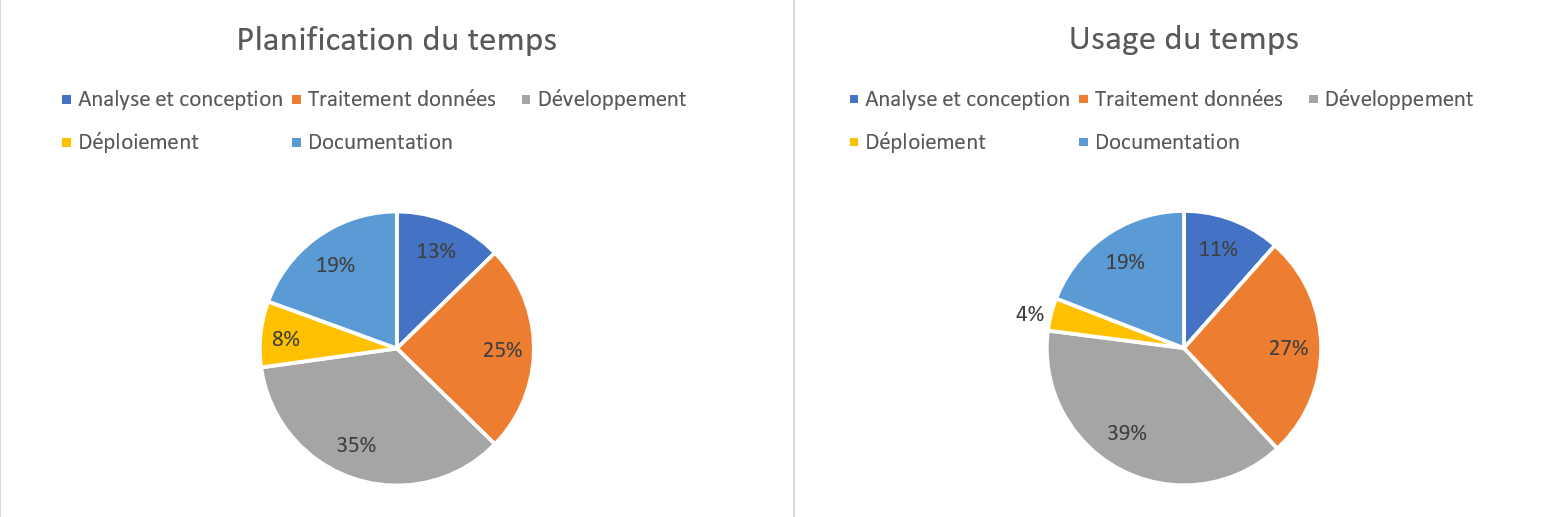
\includegraphics[scale=0.4]{RepartitionTemps.png}
    \caption{Répartition du temps}
    \label{fig:temps}
\end{figure}

A la Figure \ref{fig:temps}, on observe que le temps de travail a été plus concentré sur le traitement des données et le développement et moins sur le déploiement.


\section{Implémentations futures}
Ce projet peut être étendu de plusieurs manières.
D'abord en améliorant les différentes fonctionnalités présentes dans cette solution,
ensuite en implémentant les fonctionnalités suivantes :

\begin{itemize}
    \item Recherche par critère.
    \item Affichage de la disponibilté des salles de cours.
    \item Outil d'exportation et d'impression des plans.
    \item Outil du plus court itinéraire vers une ressource ou une salle.
    \item Outil de dessin vectoriel sur les plans.
    \item Outil de rajout de ressources localisées pour les administrateurs de l'application.
    \item Localisation de l'utilisateur sur le plan.
    \item Technologie pour surveiller le trafic de l'application.
    \item Optimiser la détection par les moteurs de recherches (SEO).
\end{itemize}

Cette liste n'est pas exhaustive.

\section{Conclusion personnelle}
Le travail accompli est, à mon avis, bon. Il est perfectible sur de nombreux points.
Pour autant, il s'agit du travail d'une seule personne, ne connaissant initialement que peu de choses dans le domaine des \gls{websig}.

Un tel projet, pour être finalisé, devrait soit être réalisé par une équipe de différents corps de métier,
et être planifié sur une période plus longue, permettant un apprentissage plus approfondi des différents domaines.

\vfil
\hspace{8cm}\makeatletter\@author\makeatother\par
\hspace{8cm}\begin{minipage}{5cm}
    %%if
    % Place pour signature numérique
    \printsignature
    %%fi
\end{minipage}
\clearpage

\appendix
\appendixpage
\addappheadtotoc

\chapter{Planning}

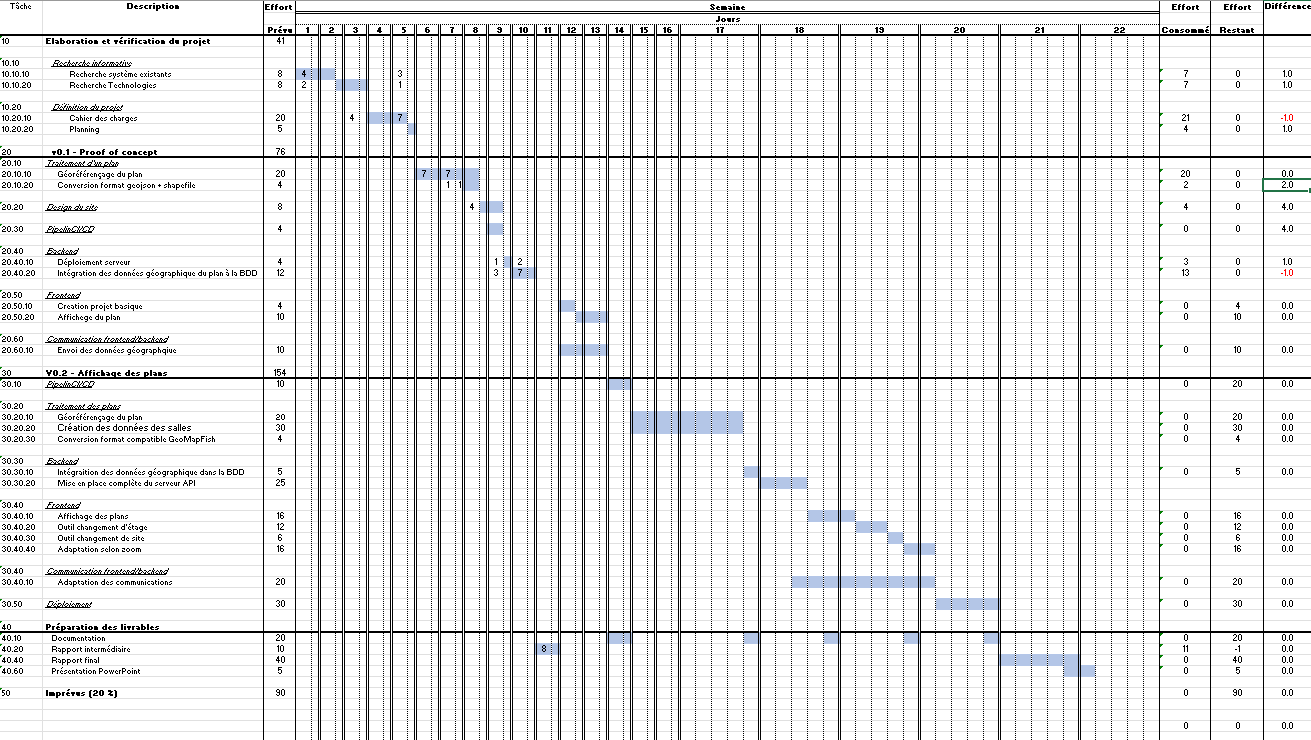
\includepdf[landscape, pages=-]{planning.pdf}

\chapter{Cahier des charges}

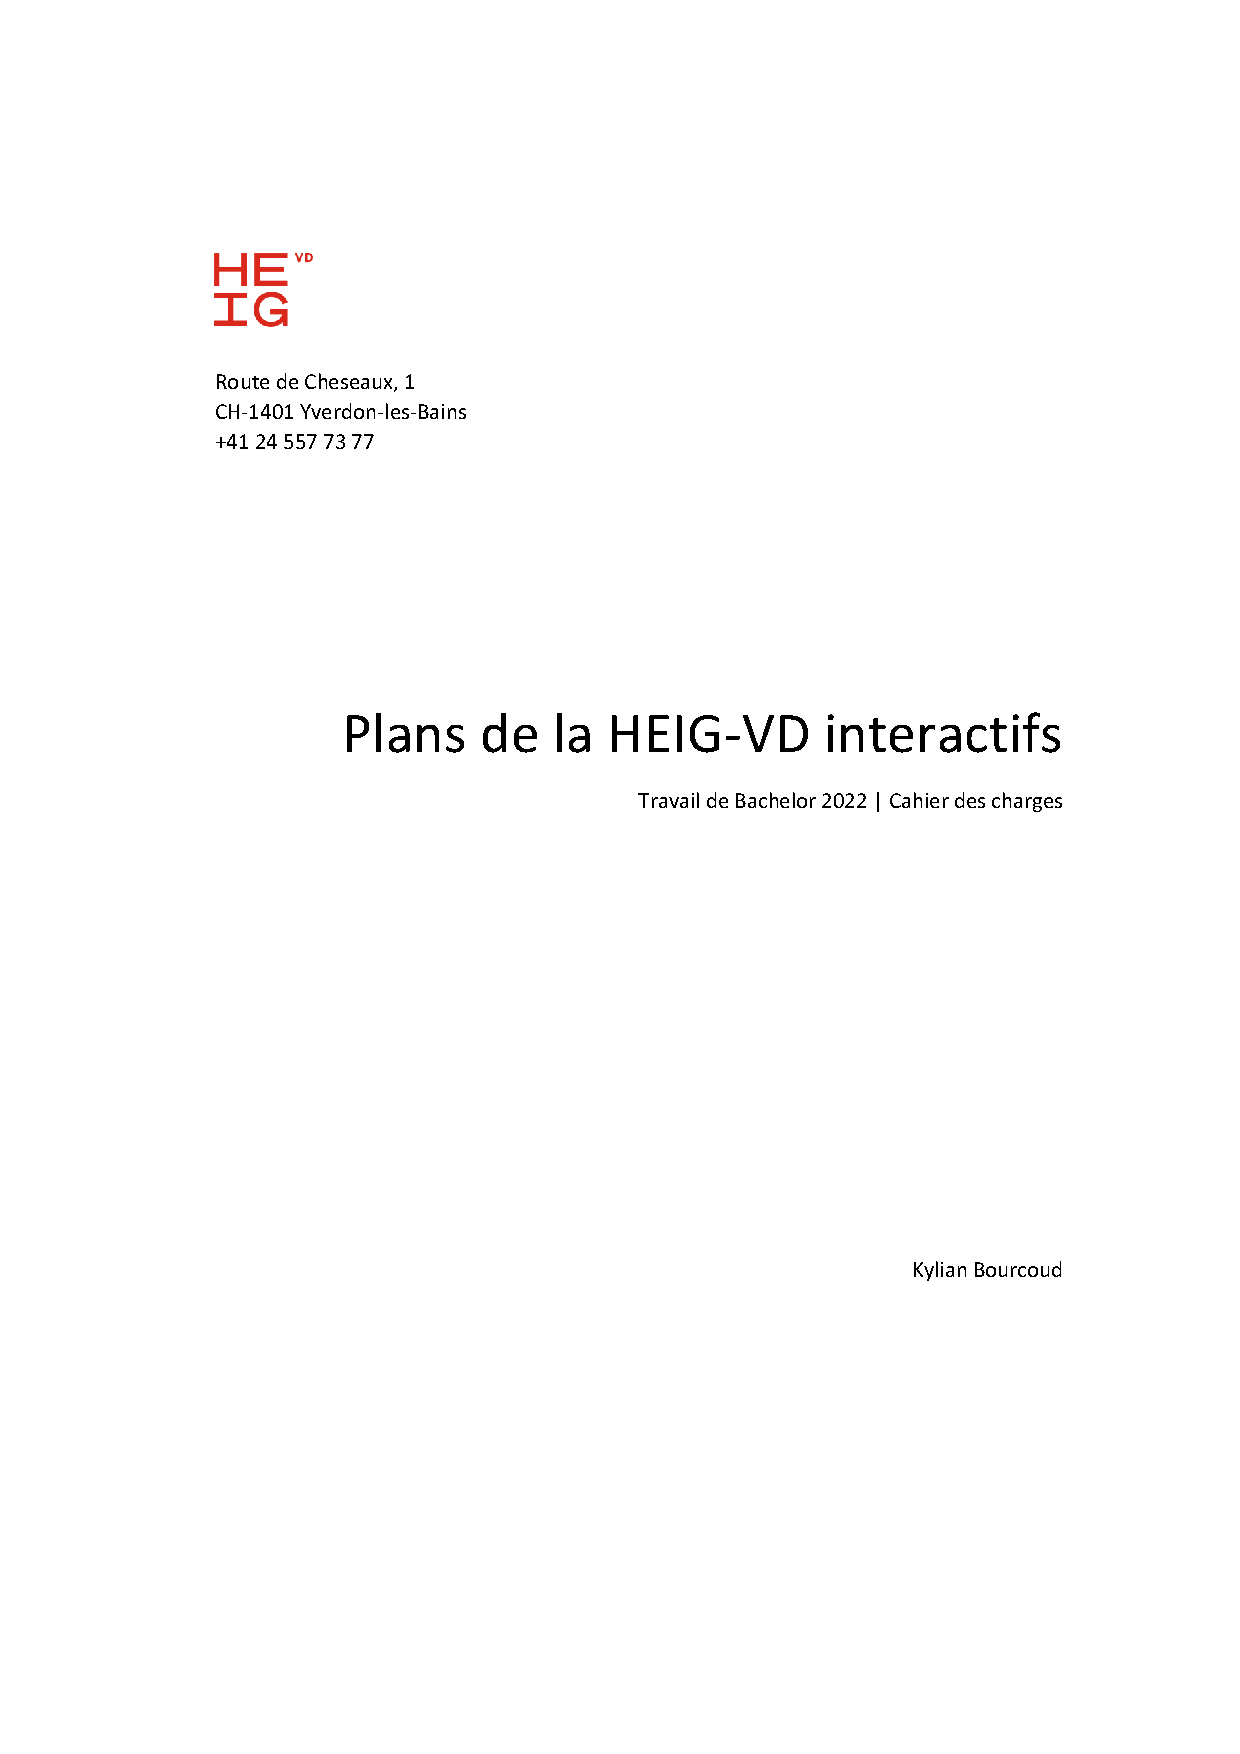
\includepdf[pages=-]{cahier_des_charges.pdf}

\let\cleardoublepage\clearpage
\backmatter

\label{glossaire}
\printnoidxglossary
\printbibliography
\label{index}
\printindex

\end{document}
